% A beamer template for AMCG
% For questions email simon.funke@gmail.com

\documentclass[	%ucs,	% loads unicode pages 0 and 1, passes correct options to the hyperref package
	%smaller,% 10pt
	bigger, % 12pt
	%draft,
	hyperref, % options for the hyperref package
	xcolor,	% xcolor package	
	%c,		% makes text in a frame vertically centered
	t,		% makes text in a frame top aligned
	%compress,	% makes navigation bars as small as possible
	%trans,	% uses the trans overlay specification
	%handout,	% sets options to be suitable for a handout
	%notes,	% hide (default), show, only or onlyslideswithnotes. Defines how notes should be handled by beamer
]{beamer}

% AMCG Theme:
\usetheme{amcg}

% UK-English
\usepackage[english]{babel}
\usepackage[latin1]{inputenc}
\usepackage[babel]{csquotes}
% \usepackage{times}
% \usepackage[T1]{fontenc}
% Or whatever. Note that the encoding and the font should match. If T1
% does not look nice, try deleting the line with the fontenc.

\usepackage{textcomp}

%% Math packages
%%\usepackage[intlimits,sumlimits]{amsmath}	% set limits correctly
% \usepackage{amsmath,amssymb,amstext,amsfonts}	% standard ams packages
% \usepackage{mathtools,mathrsfs,amsthm,units}
\usepackage{amsmath}
\usepackage{amssymb}
\usepackage{amstext}
\usepackage{amsfonts}
\usepackage{mathrsfs}
\usepackage{amsthm}
\usepackage{mathtools}
\usepackage{units}
% \usepackage{mathptmx} % Times for math

\usepackage{graphicx}
\usepackage{subfigure}
\usepackage{color} % Paket für Farben im PDF

% PGF:
\usepackage{tikz}
% \usepackage{pgfplots}
\usepackage{pgfplotstable}
% recommended:
\usepackage{booktabs}
\usepackage{array}
\usepackage{colortbl}

% For including movie:
%\usepackage{movie15}
\usepackage{multimedia}
%\usepackage{hyperref}


\usepackage{listings}
\lstset{language=Python}	% Identify programming language
\lstset{
    nolol=false,		% prints listings in listoflistings
    numberbychapter=false	% number of listings by chapter
    extendedchars=false,	% all international characters are allowed, could cause problems
    basicstyle=\small\ttfamily,% print whole listing small
    keywordstyle=\color{red!50!black}\bfseries,% bold magenta keywords
%    identifierstyle=\\bfseries,          % nothing happens
    commentstyle=\color{blue}\small\textit, % green comments
    showstringspaces=false,     % no special string spaces
    escapeinside={(*@}{@*)},	% for referencing a linenumber
%     fancyvrb=true		% load fancy verbatims package
    numbers=left,		% numbering on left side of code
    stepnumber=1,		% numbering stepsize = 1
    backgroundcolor=\color{gray!30},
    numberstyle=\tiny,		% tiny numbers
    breaklines=true,		% breaks lines automatically
    frame=tb
}

% PDF options:
\usepackage{hyperref}
\hypersetup{pdfauthor=Frank Milthaler}
\subject{FSI Modelling}

% Titlepage:
\author{Frank Milthaler}
% 
% \institute{\inst{1} Department of Earth Science and Engineering, Imperial College London}
% \and \inst{2} Centre for Navel Contemplation, Some second-rate outfit}
\date{\today}
\title[Fluid-Solid Interaction Modelling]{Fluid-Solid Interaction Modelling in Fluidity}
% \subtitle[Kurzform]{Short title}


% \usecolortheme{dolphin}
\useoutertheme{tree}
% \useinnertheme{circles}


% \newcommand\amcg{A\kern-0.25exM\kern-0.25exC\kern-0.2exG}
\newcommand\amcg{AMCG}
% Fluid velocity:
\newcommand\uf{u_f}
\newcommand\uff{u_f^f}
\newcommand\ufs{u_f^s}
\newcommand\ufhat{\hat{u}_f}
\newcommand\uffhat{\hat{u}_f^f}
% Solid velocity:
\newcommand\us{u_s}
\newcommand\uss{u_s^s}
\newcommand\usf{u_s^f}
\newcommand\ushat{\hat{u}_s}
\newcommand\usfhat{\hat{u}_s^f}
\newcommand\usbar{\bar{u}_s}
\newcommand\ussbar{\bar{u}_s^s}
\newcommand\usfbarhat{\hat{\bar{u}}_s^f}
% Alpha:
\newcommand\alphas{\alpha_s}
\newcommand\alphasf{\alphas^f}
\newcommand\alphaf{\alpha_f}
\newcommand\alphaff{\alphaf^f}
% Bulk velocity:
\newcommand\ubulk{u}
\newcommand\ubulkf{u^f}
\newcommand\ubulks{u^s}
% dt:
\newcommand\dt{\Delta t}
\newcommand\dtf{\Delta t_f}
\newcommand\dts{\Delta t_s}
% Forces:
\newcommand\Fff{F_f^f}
\newcommand\Fss{F_s^s}
\newcommand\Fsup{F^{sup}}
\newcommand\Ffsup{F_f^{sup}}
\newcommand\Fssup{F_s^{sup}}


\begin{document}

%%%%%%%%%%%%%%%%%%%%%%%%%%%%%%%%%%%%%%%%%
% Titlepage                             %
%%%%%%%%%%%%%%%%%%%%%%%%%%%%%%%%%%%%%%%%%
\begin{frame}
 \titlepage
\end{frame}

%%%%%%%%%%%%%%%%%%%%%%%%%%%%%%%%%%%%%%%%%
% Outline                               %
%%%%%%%%%%%%%%%%%%%%%%%%%%%%%%%%%%%%%%%%%
\begin{frame}{Outline}
  \tableofcontents%[pausesections]
  % You might wish to add the option [pausesections]
\end{frame}



\section{Motivation}
%%%%%%%%%%%%%%%%%%%%%%%%%%%%%%%%%%%%%%%%%
% Motivation                            %
%%%%%%%%%%%%%%%%%%%%%%%%%%%%%%%%%%%%%%%%%
\begin{frame}{Motivation}
  % - A title should summarize the slide in an understandable fashion
  %   for anyone how does not follow everything on the slide itself.
\only<1>{ \begin{itemize}
  \item Fluid-Solid Interaction Modelling
  \item Flow past turbines (wind/tidal), small scale and large scale
%   \item Von Karman vortex street
 \end{itemize}}

\only<2>{ \begin{itemize}
  \item Fluid-Solid Interaction Modelling
  \item Flow past turbines (wind/tidal), small scale and large scale
  \item Moving bodies in fluids, e.g.~turbines, vehicles
%   \item Von Karman vortex street
 \end{itemize}}

\only<3>{ \begin{itemize}
  \item Fluid-Solid Interaction Modelling
  \item Flow past turbines (wind/tidal), small scale and large scale
  \item Moving bodies in fluids, e.g.~turbines, vehicles
%   \item Von Karman vortex street
  \item Arbitrary unstructured mesh
  \item Mesh adaptivity in FSI
  \item Conservative projection between solid/fluid mesh
 \end{itemize}}

\end{frame}




%%%%%%%%%%%%%%%%%%%%%%%%%%%%%%%%%%%%%%%%%
% Branch on Launchpad                   %
%%%%%%%%%%%%%%%%%%%%%%%%%%%%%%%%%%%%%%%%%
\section{How to get it}
\begin{frame}{Branch on Launchpad}

\begin{itemize}
  \item Code is hosted as a branch of Fluidity on Launchpad
%   \item \fbox{\lstinline{bzr branch lp:~f-milthaler/fluidity/fsi-model}}
  \item Checkout: \lstinline{bzr branch lp:~f-milthaler/fluidity/fsi-model-sidebranch fluidity-fsi-model}
  \pause
  \item \lstinline{cd fluidity-fsi-model}
  \item \lstinline{module load petsc-gcc4}
  \item \lstinline{./configure --enable-2d-adaptivity && make clean && make && make fltools}
  \pause
  \item Code/Project is still under development
  \item Currently no documentation available
  \item Will be merged into the trunk in the future
\end{itemize}

\end{frame}






%%%%%%%%%%%%%%%%%%%%%%%%%%%%%%%%%%%%%%%%%
% Governing Equations                   %
%%%%%%%%%%%%%%%%%%%%%%%%%%%%%%%%%%%%%%%%%
\section{Governing Equations}

\begin{frame}{Governing Equations}
 Momementum Equation and Continuity Equation
 \begin{gather}
  \rho_f\left(\frac{\partial u}{\partial t} + u\cdot\nabla u\right) = -\nabla p + \nabla\cdot\tau + B +F_s \\
%  \nabla\cdot u + \frac{\partial \alpha_s}{\partial t} = 0
  \nabla\cdot u = 0
 \end{gather}
with
 \begin{gather}
   F_s = \sigma_f \left( u_s - u\right)
 \end{gather}
in which $\sigma_f = \dfrac{\alpha_s\rho_f}{\Delta t}$ and $\alpha_s$ being the solid volume fraction on the fluid mesh
\end{frame}



%%%%%%%%%%%%%%%%%%%%%%%%%%%%%%%%%%%%%%%%%
% Projection                            %
%%%%%%%%%%%%%%%%%%%%%%%%%%%%%%%%%%%%%%%%%
\section{Projection}
% Galerkin projection via supermesh (for mesh adaptivity):
\begin{frame}{Projection}
\only<1>{
 \begin{itemize}
  \item Galerkin projection via supermeshing\footnote{\scriptsize Farrell, Piggott et al.: \textsl{Conservative interpolation between unstructured meshes via supermesh construction};\\and Farrell, Maddison: \textsl{Conservative interpolation between volume meshes by local Galerkin projection}}
 \end{itemize}
}
\only<2>{
Donor and target mesh of same domain\footnote[2]{Graphic taken from: Farrell, PhD Thesis, \textsl{Galerkin projection of discrete fields via supermesh construction}}
 \begin{figure}[ht!]
  \centering
  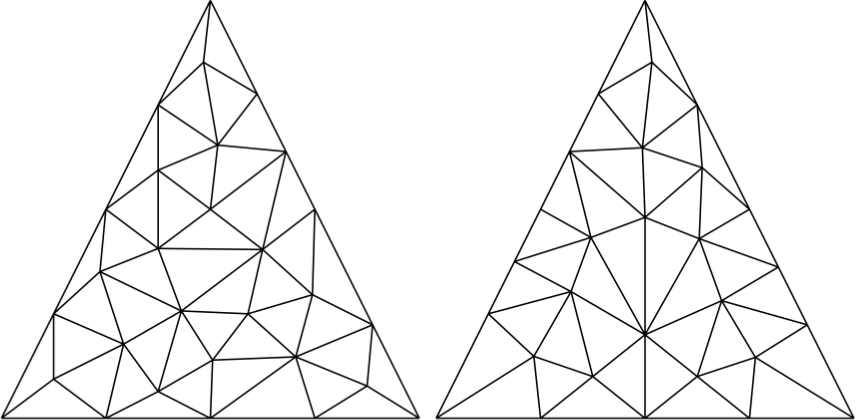
\includegraphics[scale=0.25]{content/projection/images/supermesh-input-meshes-farrell}
 \end{figure}
}
\only<3>{
Supermesh with the elements of the target mesh being coloured\footnote[2]{Graphic taken from: Farrell, PhD Thesis, \textsl{Galerkin projection of discrete fields via supermesh construction}}
 \begin{figure}[ht!]
  \centering
  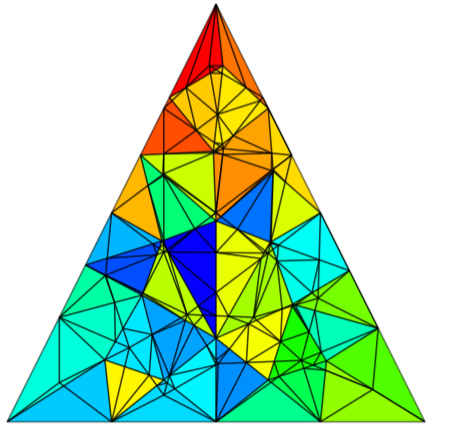
\includegraphics[scale=0.25]{content/projection/images/supermesh-supermesh-for-target-mesh-farrell}
 \end{figure}
}

\end{frame}
\begin{frame}{Projection}
 \begin{itemize}
  \item Galerkin projection via supermeshing\footnote{\scriptsize Farrell, Piggott et al.: \textsl{Conservative interpolation between unstructured meshes via supermesh construction};\\and Farrell, Maddison: \textsl{Conservative interpolation between volume meshes by local Galerkin projection}}
  \item Conservative projection of fields between meshes
  \item Bounded (with minimal numerical diffusion) or not bounded
  \pause
  \item Local supermesh of intersecting elements
  \pause
  \item Originally developed for mesh adaptivity methods: Projecting fields from old mesh to new (adapted) mesh
 \end{itemize}
\end{frame}

% Galerkin projection via Supermesh for FSI modelling:
\begin{frame}{Projection: FSI}
\only<1-4>{
 Usage of Galerkin projection via supermesh for FSI modelling:
 \begin{itemize}
  \item $\tau_F$, $\tau_S$: Fluid and Solid volume meshes of the domains $\Omega_F$, $\Omega_S$, and elements $K_F$ and $K_S$ respectively%, and nodes $N_F$ and $N_S$.
  \pause
  \item Typically: $\Omega_F \supseteq \Omega_S$
  \item Thus, some $K_F \cap K_S$ are of measure zero
  \pause
  \item Supermesh is constructed for any $K_S$ for which $K_S \cap K_F$ of nonzero measure
  \pause
  \item Must be bounded!
%   \item Element of Supermesh: $K_{Su} = \tau_S \cap \tau_F$, 
 \end{itemize}
}
\only<5>{
 \begin{figure}
  \centering
  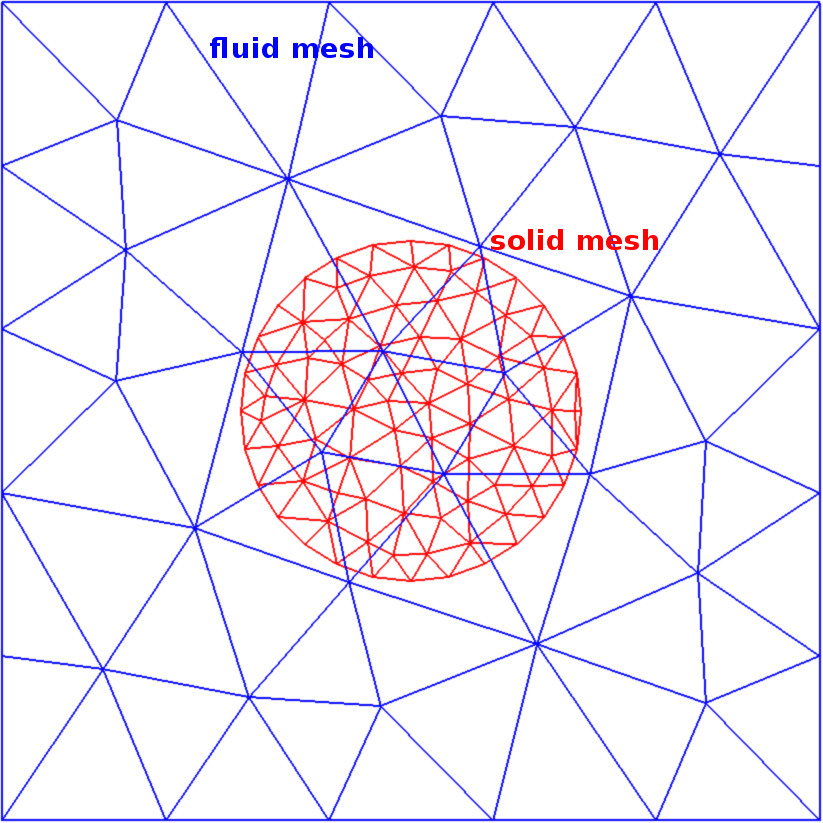
\includegraphics[scale=0.15]{content/projection/images/mesh}
 \end{figure}
}

\only<6>{
 \begin{figure}
  \centering
  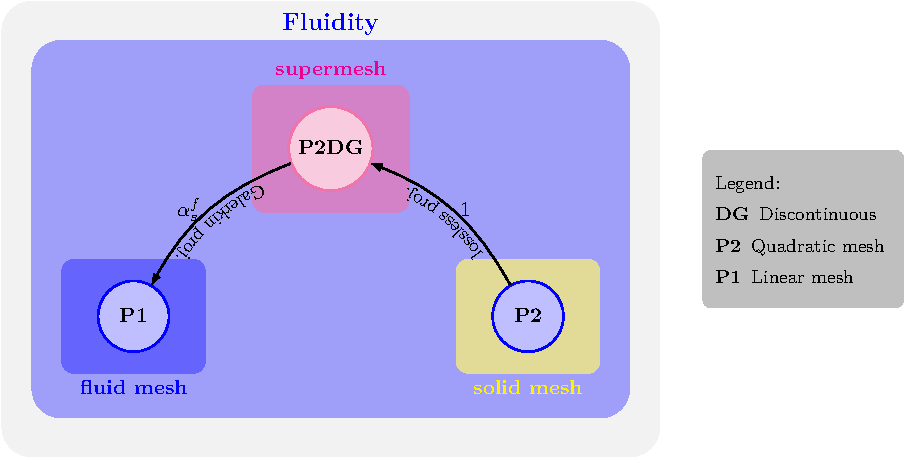
\includegraphics[width=0.9\textwidth]{content/projection/images/crop_schematic_1way_interpolation}
 \end{figure}
}
\end{frame}


%  Projection between solid and fluid mesh:
\begin{frame}{Projection: FSI}
\only<1>{
Unbounded projection:
\begin{figure}
  \centering
  \fbox{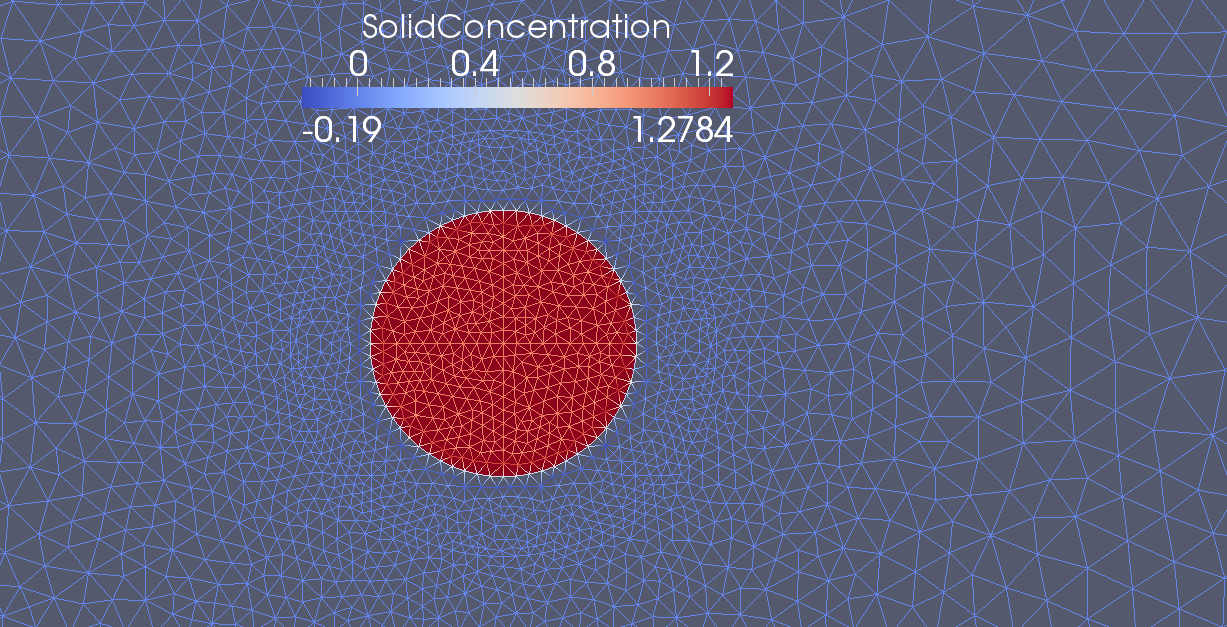
\includegraphics[scale=0.215]{content/projection/images/solid_concentration-unbounded-projection}}
 \end{figure}
}
\only<2>{
Unbounded projection:
\begin{figure}
  \centering
  \fbox{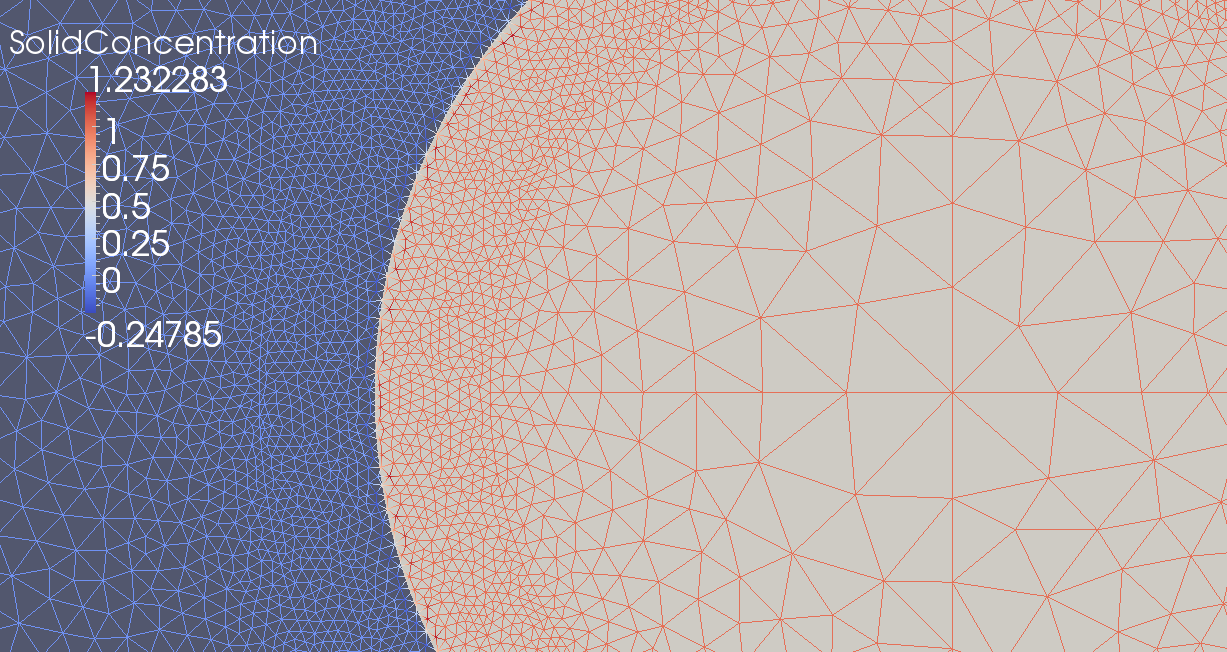
\includegraphics[scale=0.215]{content/projection/images/solid_concentration-unbounded-projection-zoom}}
 \end{figure}
}
\only<3>{
Bounded projection:
 \begin{figure}
  \centering
  \fbox{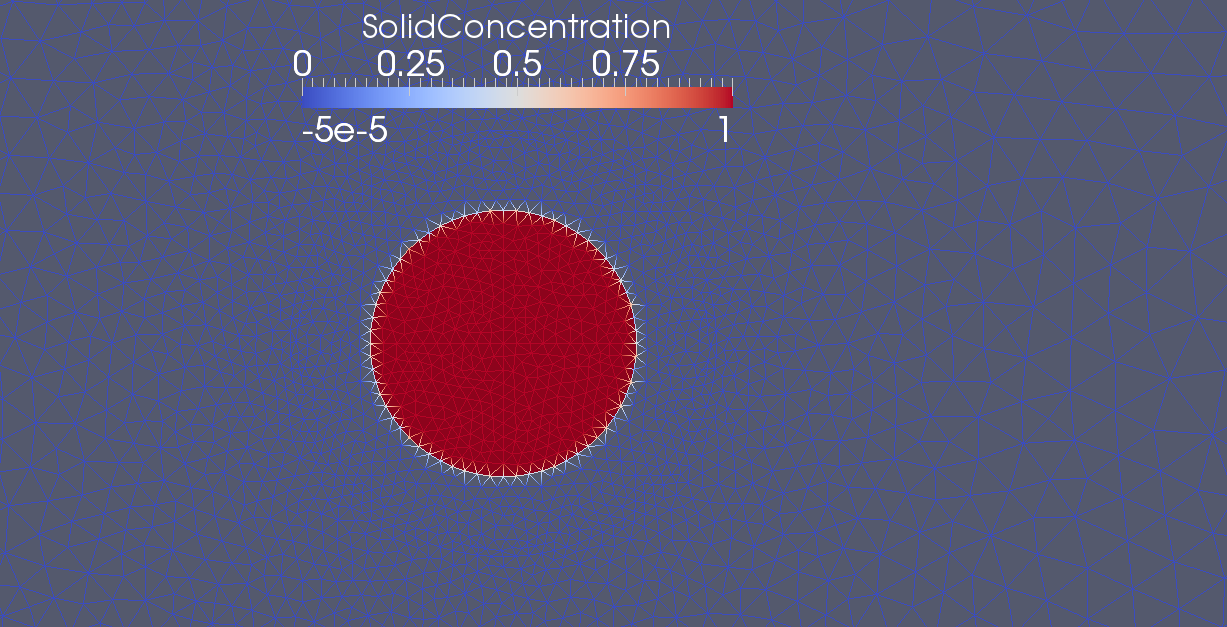
\includegraphics[scale=0.215]{content/projection/images/solid_concentration-bounded-projection}}
 \end{figure}
}
\only<4>{
Bounded projection:
 \begin{figure}
  \centering
  \fbox{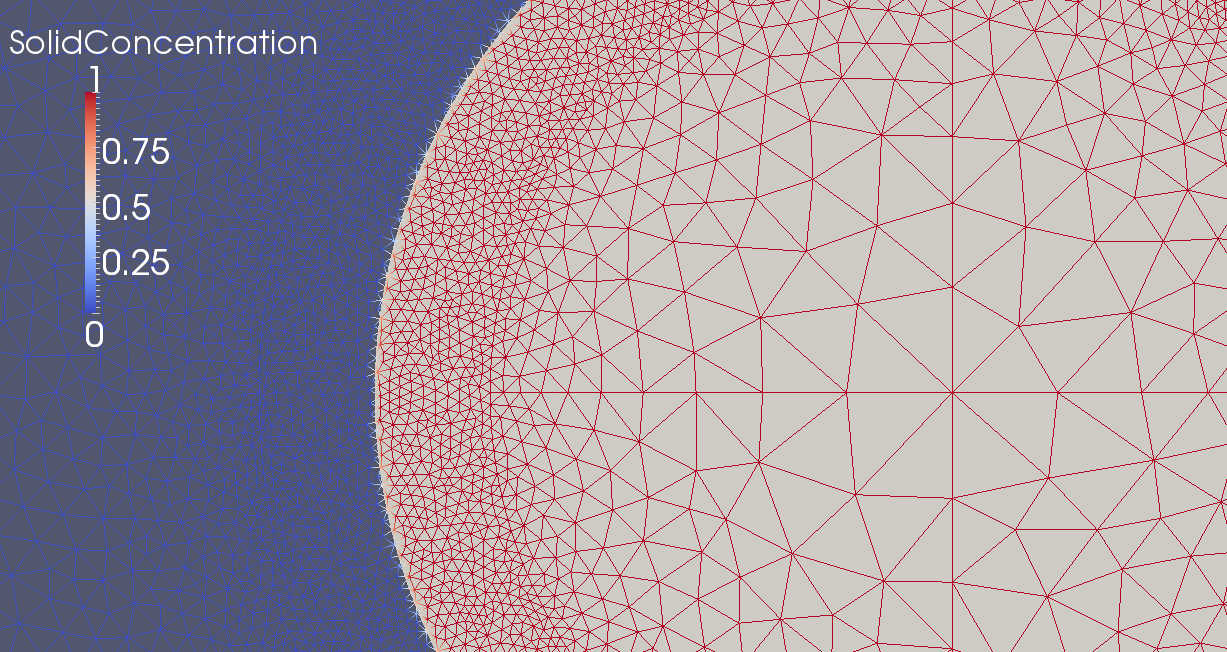
\includegraphics[scale=0.215]{content/projection/images/solid_concentration-bounded-projection-zoom}}
 \end{figure}
}
\end{frame}



%%%%%%%%%%%%%%%%%%%%%%%%%%%%%%%%%%%%%%%%%
% Projection                            %
%%%%%%%%%%%%%%%%%%%%%%%%%%%%%%%%%%%%%%%%%
\section{Mesh Adaptivity and FSI}

\begin{frame}{Mesh Adaptivity for FSI}
 Mesh adaptivity is very useful for FSI modelling:
 \begin{itemize}
  \item Refining the area of interest, e.g.~space around the solid body
  \item Can be done as a preprocessing task to avoid manual local refinement
  \item Makes it simply to track a moving body
  \item Reduces computational effort
 \end{itemize}
\end{frame}

\begin{frame}{Mesh Adaptivity for FSI}

{\color{blue}Fluid mesh} and {\color{red}Solid meshes}
\vspace{-3ex}
\only<1>{
 \begin{figure}
  \centering
  \subfigure{{\fbox{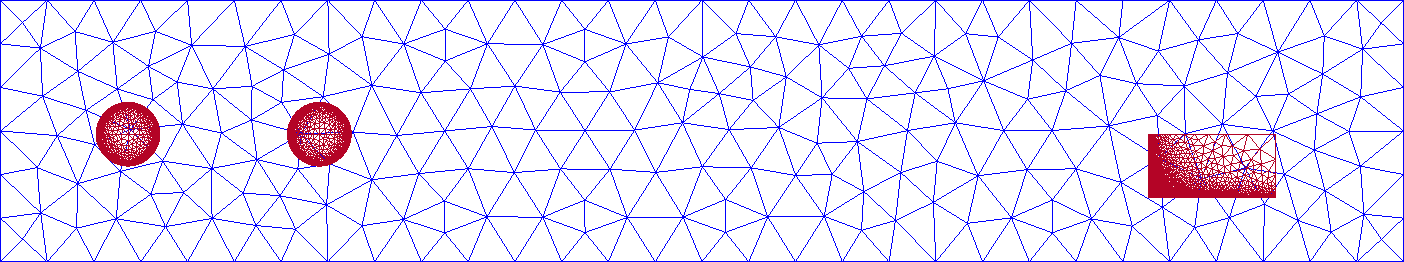
\includegraphics[scale=0.215]{content/projection/images/initial_mesh_fsi}}}}\\
 \end{figure}
}
\only<2>{
 \begin{figure}
  \centering
  \subfigure{{\fbox{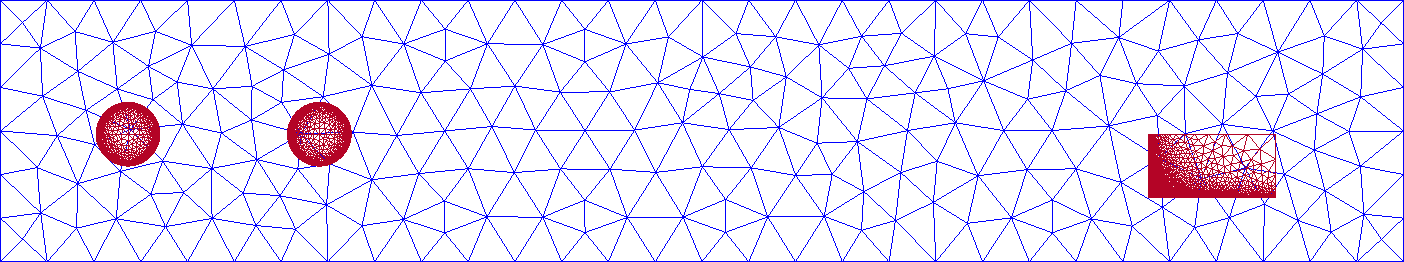
\includegraphics[scale=0.215]{content/projection/images/initial_mesh_fsi}}}}\\
  \subfigure{{\fbox{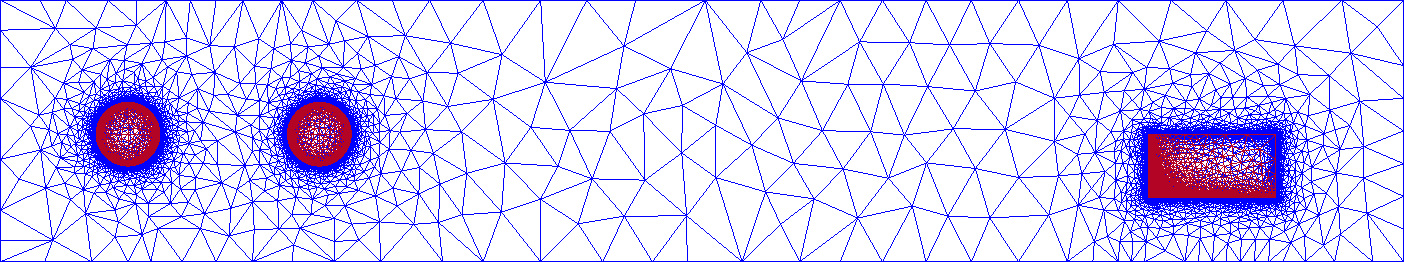
\includegraphics[scale=0.215]{content/projection/images/mesh_adaptivity_in_fsi}}}}
 \end{figure}
}
\end{frame}




%%%%%%%%%%%%%%%%%%%%%%%%%%%%%%%%%%%%%%%%%
% Applications                          %
%%%%%%%%%%%%%%%%%%%%%%%%%%%%%%%%%%%%%%%%%
\section{Applications}
% Overview of applications/validation test cases:
\begin{frame}{Applications}
 \begin{itemize}
  \item Fixed solid
  \begin{itemize}
    \item Flow past a cylinder (2D, 3D), $Re=20$ and $Re=100$
    \item Flow past a sphere, $Re=[20,5000]$
    \item Von Karman Vortex Street
    \item Flow past aerofoil
  \end{itemize}
  \pause
  \item Moving solid:
  \begin{itemize}
    \item St Andrews Cross
    \item Wind turbine, Tidal Turbine
    \item Ellipse/Ellipsoid moving through stratified fluid
  \end{itemize}
 \end{itemize}
\end{frame}

% Images of FSI modelling, with a fixed solid body:
\begin{frame}{Fixed Solid}
 \vspace{-2ex}
  \begin{figure}
  \centering
  \only<1>{\fbox{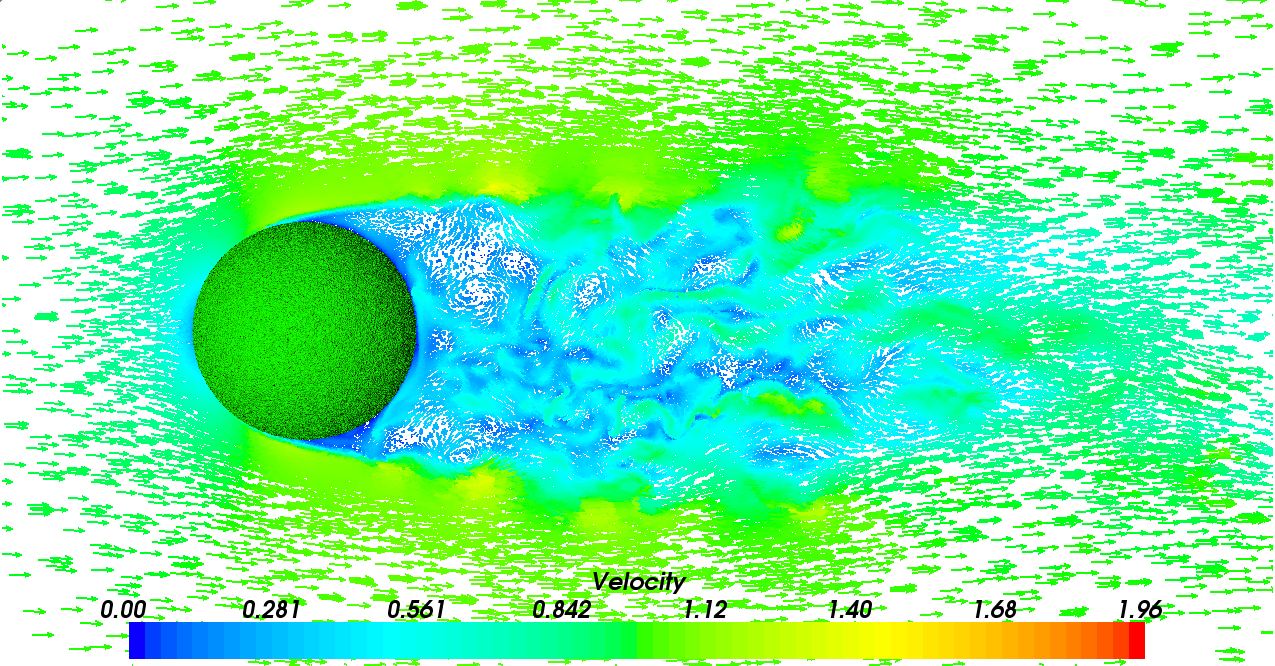
\includegraphics[scale=0.215]{content/fsi-images/re5000_sphere_legend}}}
  \only<2>{\fbox{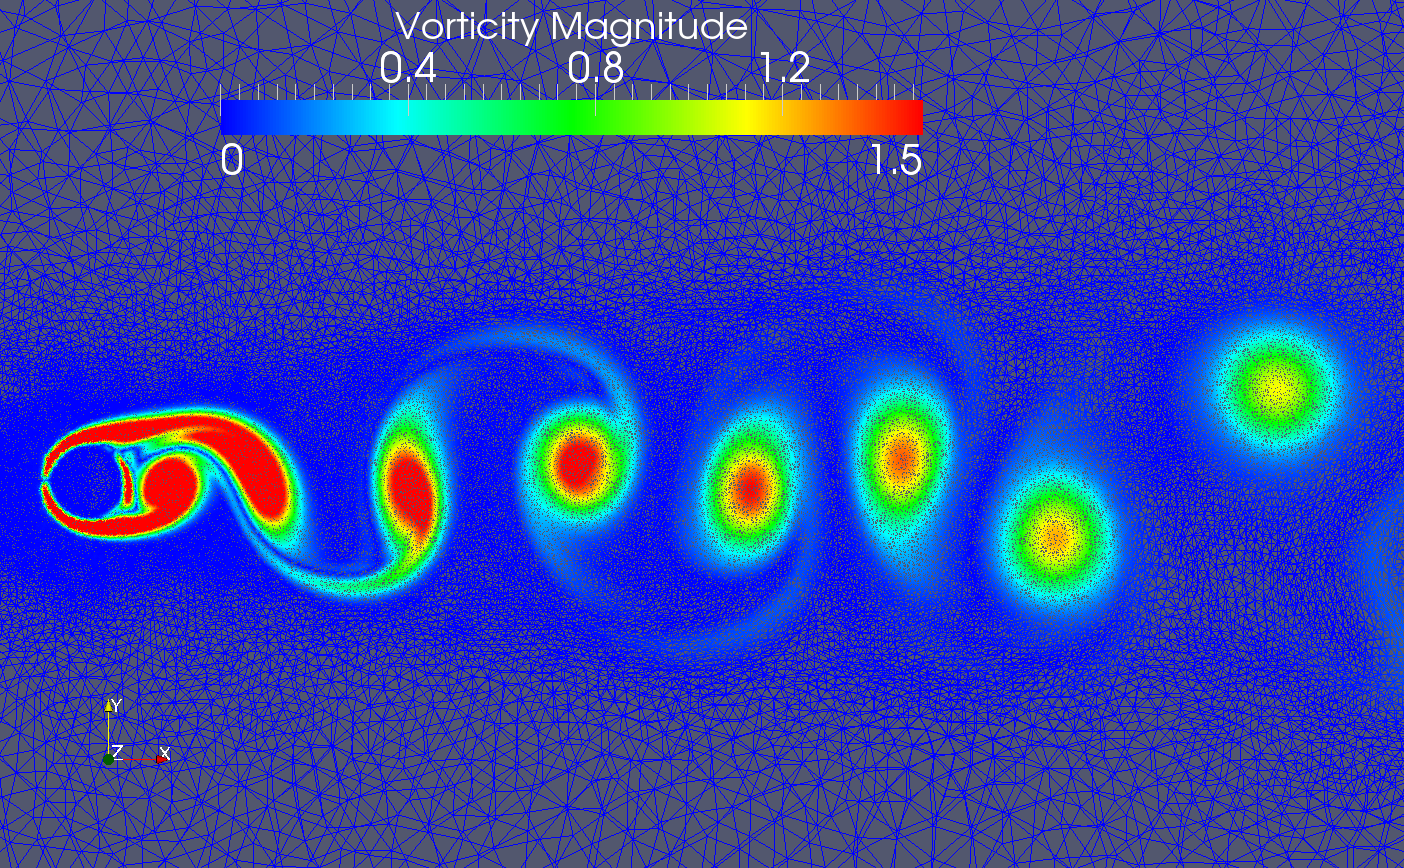
\includegraphics[scale=0.2]{content/fsi-images/von_karman_vortex_street}}}
 \end{figure}
\end{frame}

% Images of FSI modelling, with a moving solid body:
\begin{frame}{Rotating Wind Turbine}
 \vspace{-2ex}
  \begin{figure}
  \centering
  \only<1>{\fbox{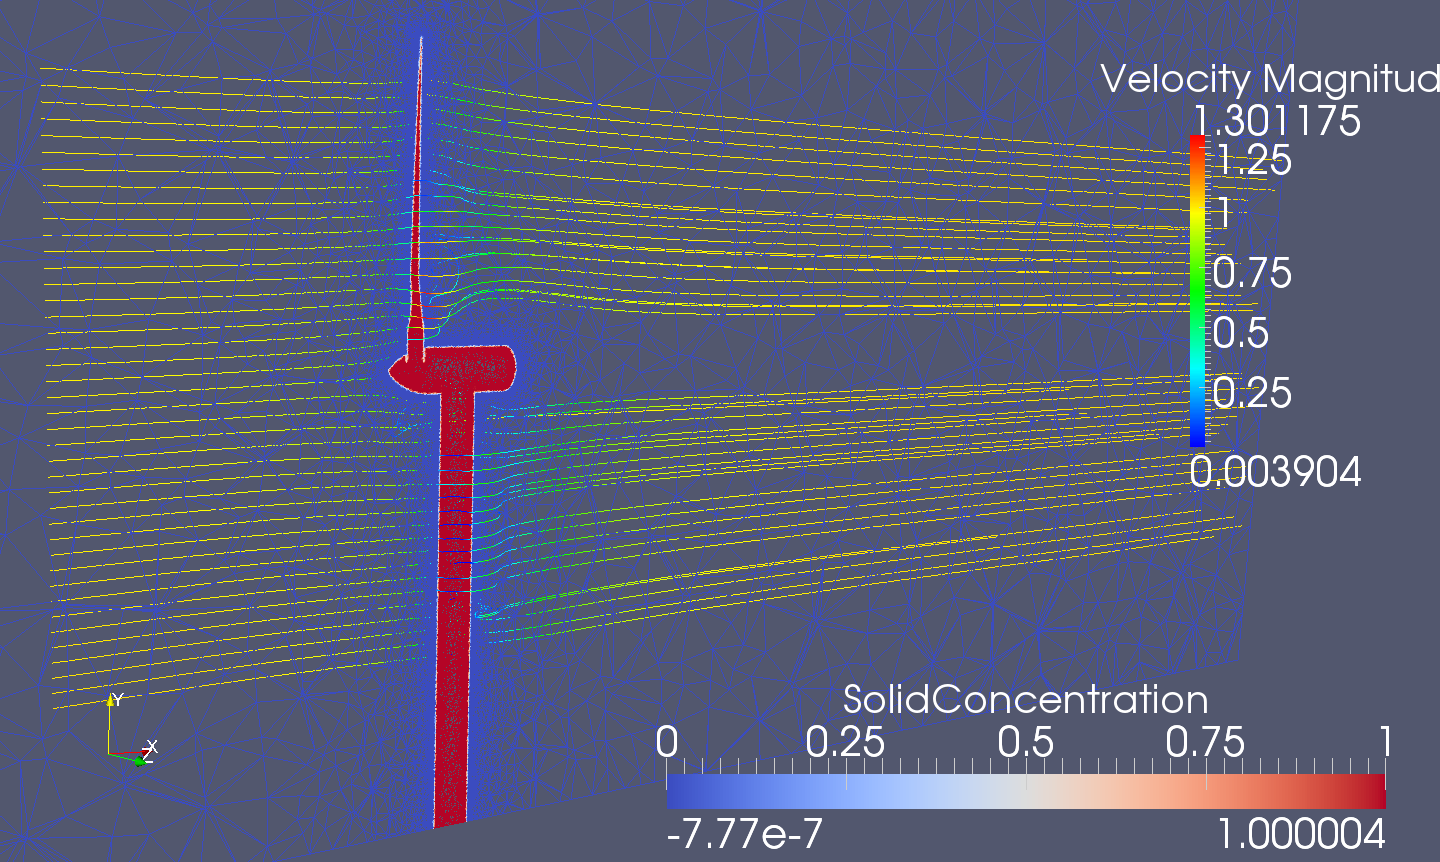
\includegraphics[width=0.8\textwidth]{content/fsi-images/flow_past_stationary_turbine-fluidmesh_cut}}}
  \only<2>{\fbox{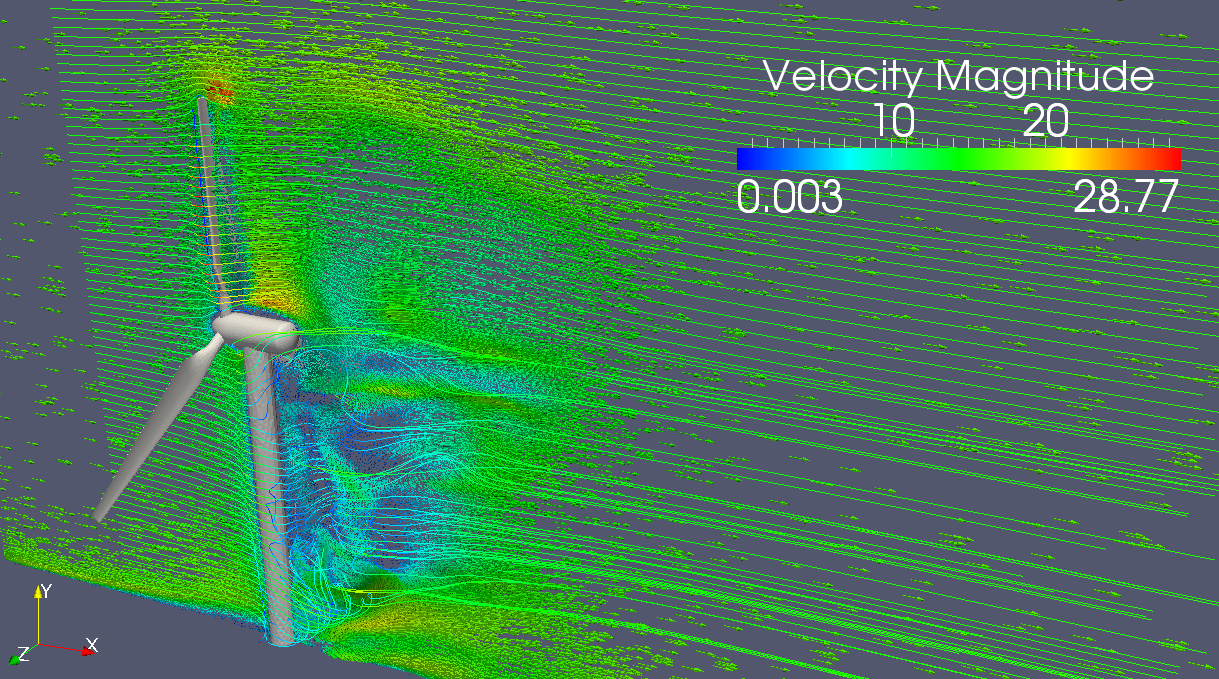
\includegraphics[width=0.8\textwidth]{content/fsi-images/back-blades-velocity-arrows-tracer}}}
  % For multimedia:
  \only<3>{\centering\movie[width=10cm,height=6cm,repeat]{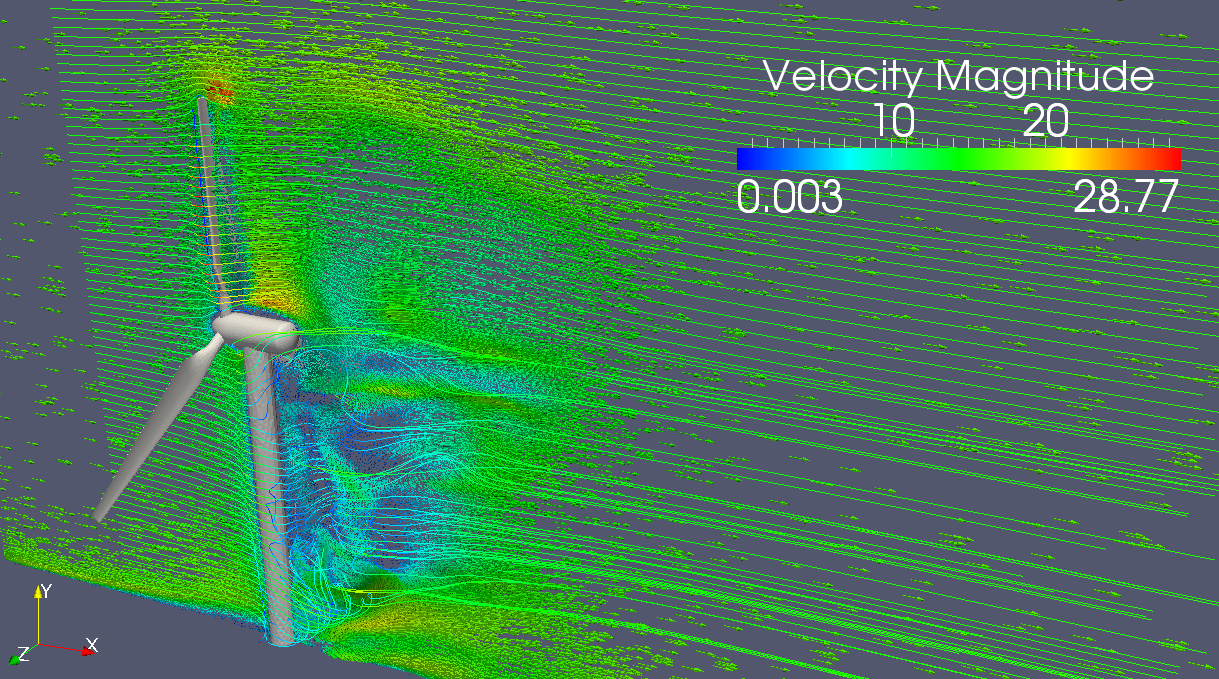
\includegraphics[width=10cm,height=6cm]{content/fsi-images/back-blades-velocity-arrows-tracer}}{content/movies/back-blades-velocity-arrow-2.avi}}
  % For hyperref:
  %\only<3>{\centering\href{run:content/movies/back-blades-velocity-arrow-2.avi}{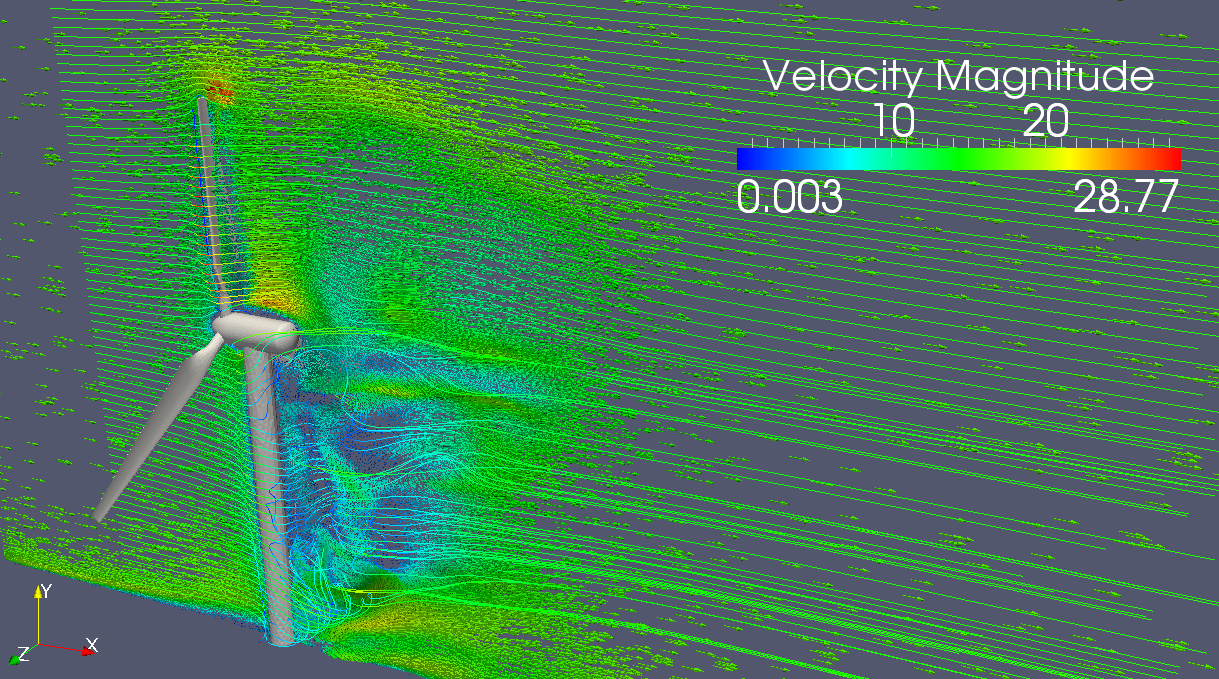
\includegraphics[width=10cm,height=6cm]{content/fsi-images/back-blades-velocity-arrows-tracer}}}
  % For movie15:
%  \only<3>{\centering\includemovie[poster={content/fsi-images/back-blades-velocity-arrows-tracer.png},mimetype=video/avi,inline=true]{}{}{content/movies/back-blades-velocity-arrow-2.avi}}
  %\only<3>{\centering\includemovie[poster,mimetype=video/avi,inline=true,text={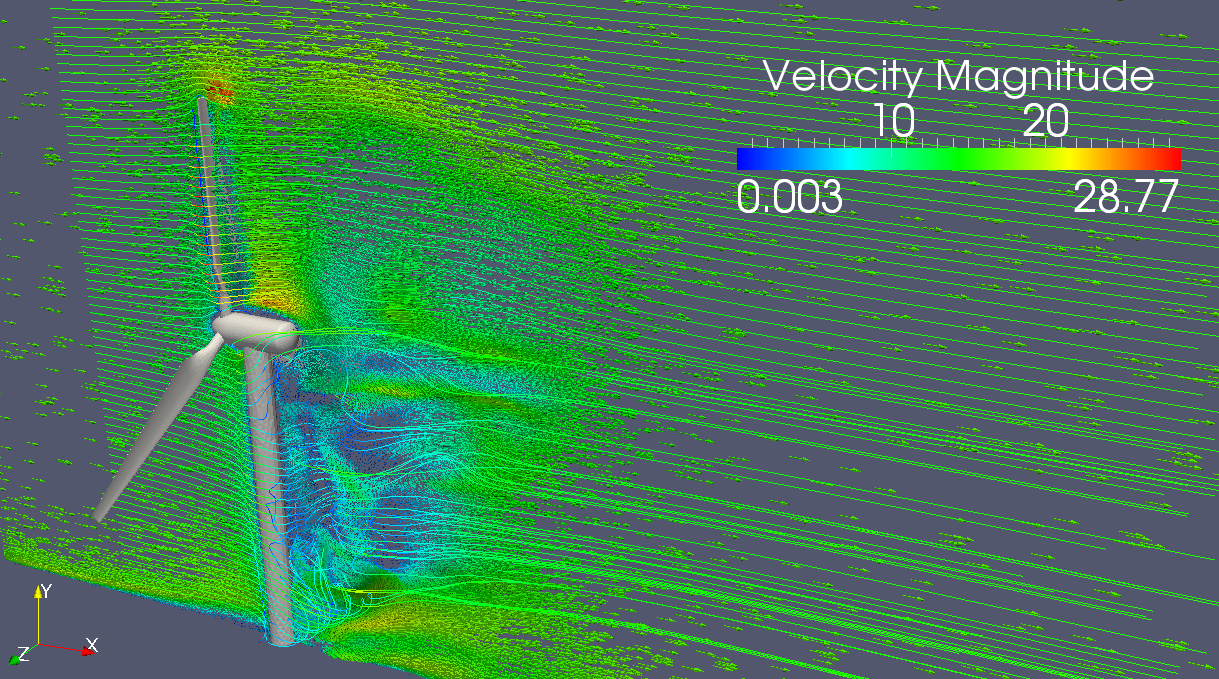
\includegraphics[width=10cm,height=6cm]{content/fsi-images/back-blades-velocity-arrows-tracer}}]{}{}{content/movies/back-blades-velocity-arrow-2.avi}}
 \end{figure}
\end{frame}

%%%%%%%%%%%%%%%%%%%%%%%%%%%%%%%%%%%%%%%%%
% St Andrews Cross                      %
%%%%%%%%%%%%%%%%%%%%%%%%%%%%%%%%%%%%%%%%%
\begin{frame}{St Andrews Cross}
 \begin{itemize}
  \item Momentum Source\footnote[3]{Javam et al, \textsl{Numerical study of internal wave reflection from sloping boundaries}}
  \item Angle of internal wave propagation:
   \begin{equation}
    \sin\alpha = \frac{\omega}{N}
   \end{equation}
   in which $\omega$ is the oscillation frequency, and $N=\left(\left(g/\rho_0\right)\left|\tfrac{d\rho}{dy}\right|\right)^{1/2}$ the buoyancy frequency, with $\rho$, $\rho_0$, and $g$ being the density, reference density, and gravitational acceleration respectively
  \item Validation for FSI with prescribed solid velocity
 \end{itemize}
\end{frame}

\begin{frame}{St Andrews Cross}
 \begin{itemize}
  \item Momentum Source\footnote[3]{Javam et al, \textsl{Numerical study of internal wave reflection from sloping boundaries}}
  \item FSI model
  \item Both with:
 \end{itemize}
 \begin{align*}
  & & \omega &= 0.699 & & & & & &\\
  & & N &= 1 & & & & & &\\
  \shortintertext{Which yields to}
  & & \alpha &= 44.347 & & & & & &
 \end{align*}
\end{frame}

\begin{frame}{St Andrews Cross}
 \vspace{-3ex}
  \begin{figure}
  \centering
  \only<1>{\fbox{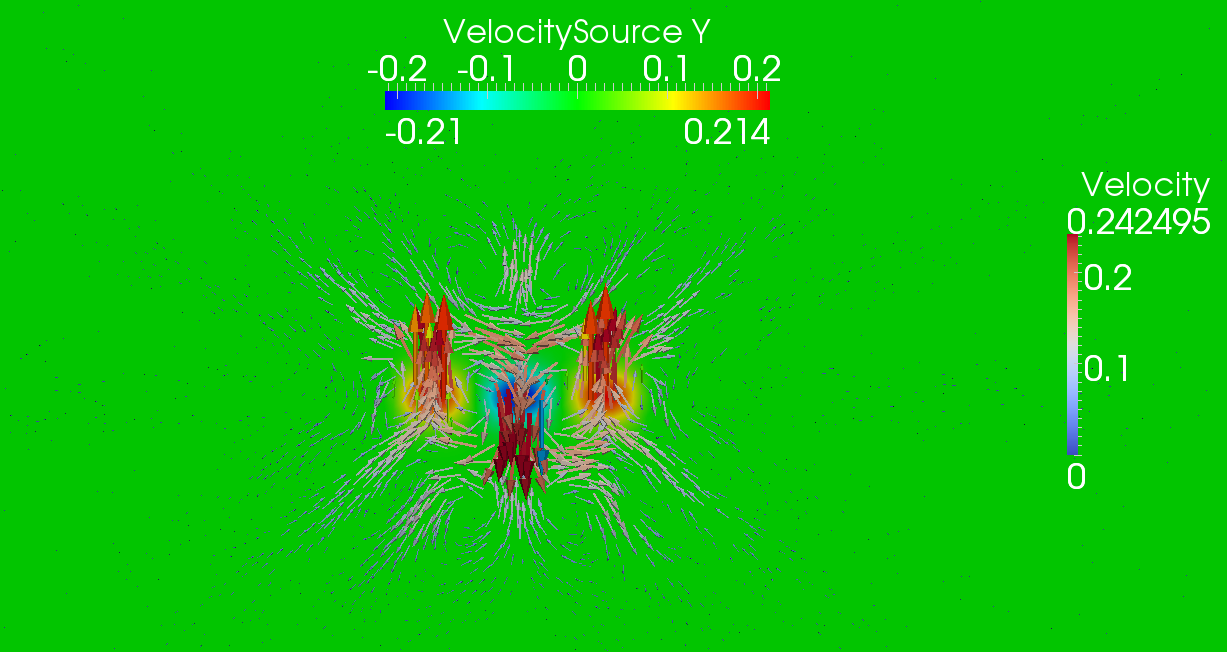
\includegraphics[width=0.8\textwidth]{content/st-andrews-cross/momentum-source/momentum-source-st-andrews-cross-fixed-newsetup-p1dgp2-el-0-2_source_and_velocity_glyphs}}}
  \only<2>{\fbox{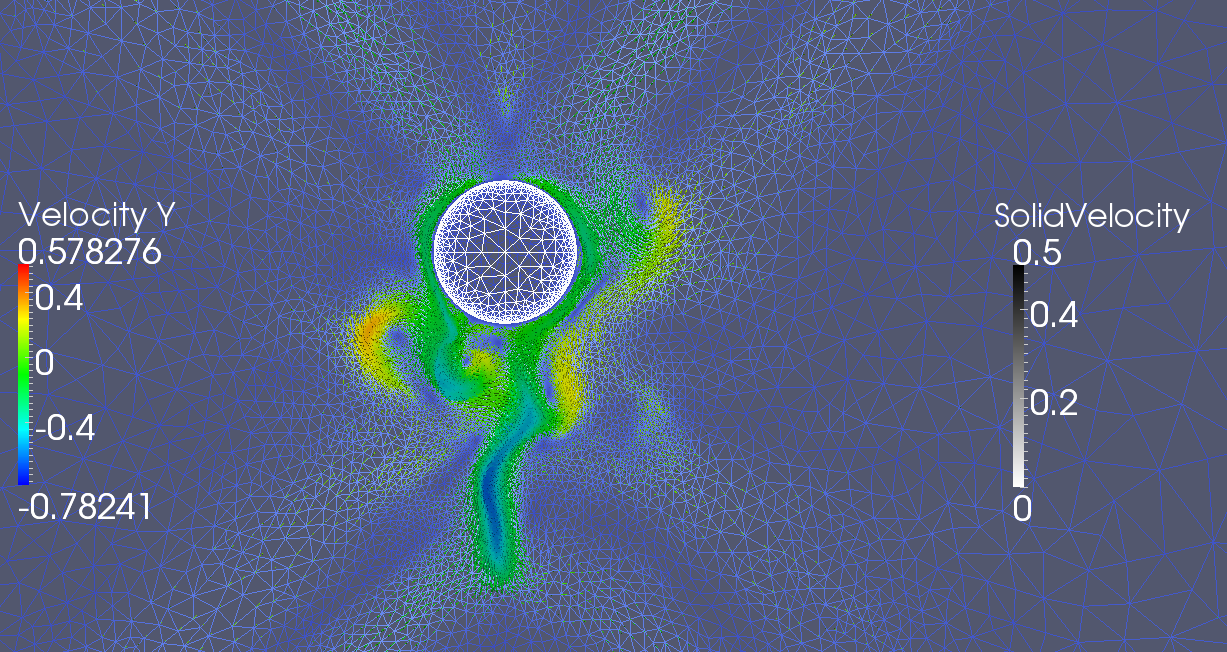
\includegraphics[width=0.8\textwidth]{content/st-andrews-cross/fsi/fsi-st-andrews-cross-tophat-adap_vely_sinv_r05_el-0-01_velocity_glyphs}}}
  % For multimedia:
  \only<3>{\centering\movie[width=11cm,height=6cm,repeat]{\includegraphics[width=10cm,height=6cm]{content/st-andrews-cross/movies/fsi-st-andrews-cross-tophat-fixed_veryfine_sinv_r05_el-0-05-startscreen}}{content/st-andrews-cross/movies/fsi-st-andrews-cross-tophat-fixed_veryfine_sinv_r05_el-0-05.avi}}
  % For hyperref:
  %\only<3>{\centering\href{run:content/st-andrews-cross/movies/fsi-st-andrews-cross-tophat-fixed_veryfine_sinv_r05_el-0-05.avi}{\includegraphics[width=10cm,height=6cm]{content/st-andrews-cross/movies/fsi-st-andrews-cross-tophat-fixed_veryfine_sinv_r05_el-0-05-startscreen}}}
  % For movie15:
  %\only<3>{\includemovie[poster,mimetype=video/avi,inline=true,text={\includegraphics[width=10cm,height=6cm]{content/st-andrews-cross/movies/fsi-st-andrews-cross-tophat-fixed_veryfine_sinv_r05_el-0-05-startscreen}}]{}{}{content/st-andrews-cross/movies/fsi-st-andrews-cross-tophat-fixed_veryfine_sinv_r05_el-0-05.avi}}
  %\only<3>{\includemovie[poster,mimetype=video/avi, inline=true]{}{}{content/st-andrews-cross/movies/fsi-st-andrews-cross-tophat-fixed_veryfine_sinv_r05_el-0-05.avi}}
  % Next video:
  % For multimedia:
  \only<4>{\movie[width=11cm,height=6cm,repeat]{\includegraphics[width=10cm,height=6cm]{content/st-andrews-cross/movies/fsi-st-andrews-cross-tophat-adap_vely_sinv_r05_el-0-01-startscreen}}{content/st-andrews-cross/movies/fsi-st-andrews-cross-tophat-adap_vely_sinv_r05_el-0-01.avi}}
  % For hyperref:
  %\only<4>{\centering\href{run:content/st-andrews-cross/movies/fsi-st-andrews-cross-tophat-adap_vely_sinv_r05_el-0-01.avi}{\includegraphics[width=10cm,height=6cm]{content/st-andrews-cross/movies/fsi-st-andrews-cross-tophat-adap_vely_sinv_r05_el-0-01-startscreen}}}
  % For movie15:
  %\only<4>{\includemovie[poster,mimetype=video/avi,inline=true,text={\includegraphics[width=10cm,height=6cm]{content/st-andrews-cross/movies/fsi-st-andrews-cross-tophat-adap_vely_sinv_r05_el-0-01-startscreen}}]{}{}{content/st-andrews-cross/movies/fsi-st-andrews-cross-tophat-adap_vely_sinv_r05_el-0-01.avi}}
  % Next video:
  % For multimedia:
  \only<5>{\movie[width=11cm,height=6cm,repeat]{\includegraphics[width=10cm,height=6cm]{content/st-andrews-cross/movies/fsi-st-andrews-cross-tophat-adap_vely_sinv_r05_el-0-01_closeup-startscreen}}{content/st-andrews-cross/movies/fsi-st-andrews-cross-tophat-adap_vely_sinv_r05_el-0-01_closeup.avi}}
  % For hyperref:
  %\only<5>{\centering\href{run:content/st-andrews-cross/movies/fsi-st-andrews-cross-tophat-adap_vely_sinv_r05_el-0-01_closeup.avi}{\includegraphics[width=10cm,height=6cm]{content/st-andrews-cross/movies/fsi-st-andrews-cross-tophat-adap_vely_sinv_r05_el-0-01_closeup-startscreen}}}
  % For movie15:
  %\only<5>{\includemovie[poster,mimetype=video/avi,inline=true,text={\includegraphics[width=10cm,height=6cm]{content/st-andrews-cross/movies/fsi-st-andrews-cross-tophat-adap_vely_sinv_r05_el-0-01_closeup-startscreen}}]{}{}{content/st-andrews-cross/movies/fsi-st-andrews-cross-tophat-adap_vely_sinv_r05_el-0-01_closeup.avi}}
 \end{figure}
\end{frame}

% St-Andrews-Cross: Validation
\begin{frame}{St Andrews Cross --- Validation}
 \vspace{-3ex}
  \begin{figure}
  \centering
  \only<1>{\vspace{3ex}\fbox{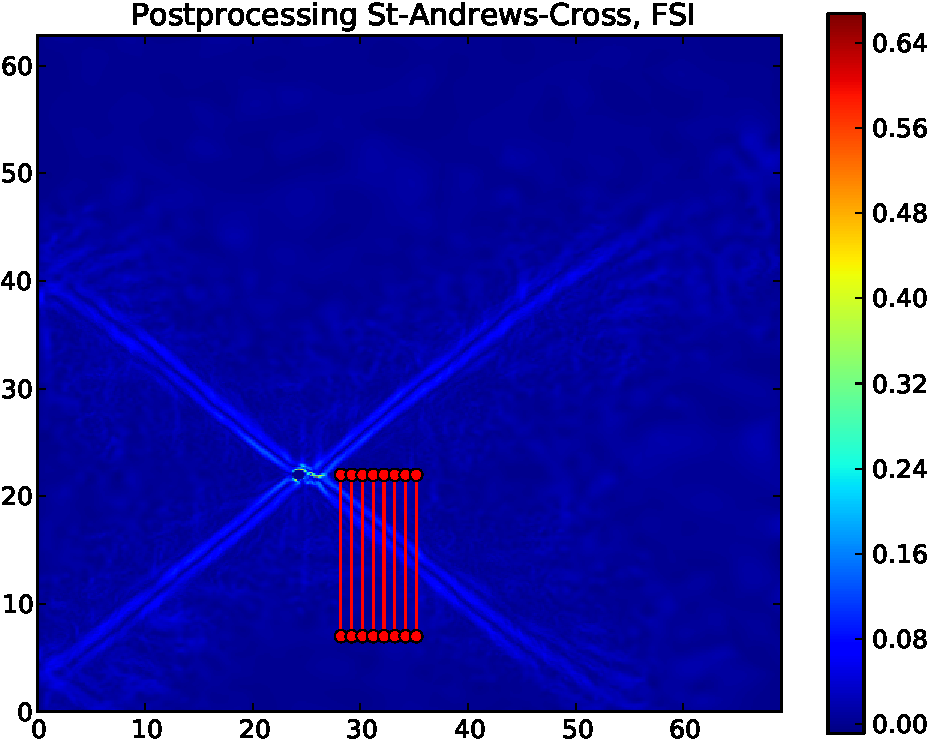
\includegraphics[scale=0.4]{content/st-andrews-cross/convergence-plots/postprocessing_st-andrews-cross_fsi}}}
  \only<2>{\fbox{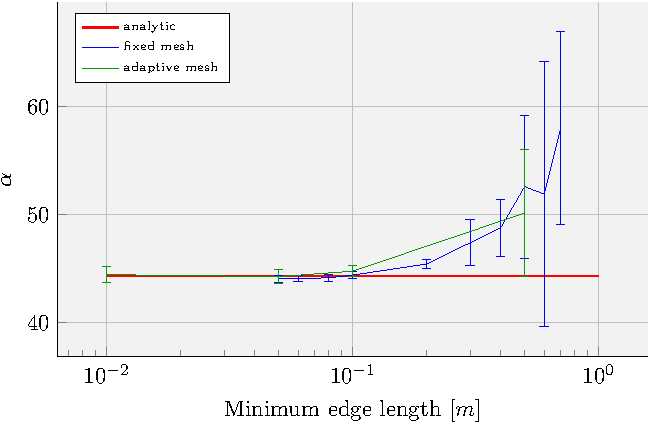
\includegraphics[width=0.8\textwidth]{content/st-andrews-cross/convergence-plots/pgfplot_texfile_st-andrews-cross_fsi_results_elmin}}}
  \only<3>{\fbox{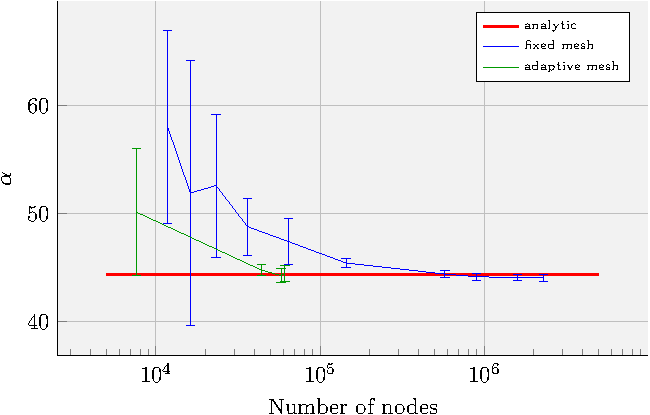
\includegraphics[width=0.8\textwidth]{content/st-andrews-cross/convergence-plots/pgfplot_texfile_st-andrews-cross_fsi_results_numnodes}}}
 \end{figure}
\end{frame}

\begin{frame}{St Andrews Cross --- Validation}
 \scriptsize
 \only<1>{% Load this file in your LaTeX document with:
% % Load this file in your LaTeX document with:
% % Load this file in your LaTeX document with:
% \input{st-andrews-cross-validation_include.tex}

% Load table settings:
\input{content/st-andrews-cross/convergence-plots/table-adaptive/pgftablesettings_st-andrews-cross-validation.tex}
% Load table data:
\pgfplotstableread{content/st-andrews-cross/convergence-plots/table-adaptive/st-andrews-cross-validation_data.pgfdat}\pgftablestandrewscrossvalidation

\begin{table}
  \centering
  \pgfplotstabletypeset[columns={elmin,num_nodes,min_sim_angle,abs_error,rel_error,angle_mean,mean_rel_error,angle_std},
  ]\pgftablestandrewscrossvalidation
  \caption{St Andrews Cross validation, adaptive mesh: $\omega = 0.699$, $N=1$, $\alpha=44.347$}%, with a prescribed velocity of the cylinder of $A\sin(\omega t)$, with $A=r=0.5$, $r$ being the radius of the cylinder, and $t$ being the time of the simulation. Shown are the minimum angle found as well as the averaged angle at all the positions the angle was computed. Note, the averaged values can be biased due to very large errors found at one distance.}
  \label{tab:st-andrews-cross-validation}
\end{table}


% Load table settings:
% PGFPlotsTable settings are defined below.
% To load them:
% \input{table/pgftablesettings_st-andrews-cross-validation.tex}

\pgfplotstableset{
    %    col sep=&,row sep=\\
    %    col sep=space, ignore chars={(,),\ ,\#}
    % Coloring:
    every even row/.style={before row={\rowcolor[gray]{0.85}}},
    % Table header:
    every head row/.style={before row=\toprule,after row=\midrule},
    every last row/.style={after row=\bottomrule},
    % Set column parameters:
    columns={simulation_name, distance, num_nodes, elmin, min_sim_angle, mean_abs_error, abs_error, rel_error, mean_rel_error, angle_std, angle_mean},
    columns/simulation_name/.style={column name=simulation name,
        string type,
        string replace={fsi-st-andrews-cross-tophat-adap_vely_sinv_r05_el-0-01}{fsi-st-andrews-cross-tophat-adap\_vely\_sinv\_r05\_el-0-01},
        string replace={fsi-st-andrews-cross-tophat-adap_vely_sinv_r05_el-0-05}{fsi-st-andrews-cross-tophat-adap\_vely\_sinv\_r05\_el-0-05},
        string replace={fsi-st-andrews-cross-tophat-adap_vely_sinv_r05_el-0-1}{fsi-st-andrews-cross-tophat-adap\_vely\_sinv\_r05\_el-0-1},
        string replace={fsi-st-andrews-cross-tophat-adap_vely_sinv_r05_el-0-5}{fsi-st-andrews-cross-tophat-adap\_vely\_sinv\_r05\_el-0-5},
        column type={l|},
    },
    columns/distance/.style={column name=distance,
        sci, sci zerofill,
        precision=3, fixed,
        dec sep align,
    },
    columns/num_nodes/.style={column name=No Nodes,
        sci, sci zerofill,
        precision=3, fixed,
        dec sep align,
    },
    columns/elmin/.style={column name=Min el,
        sci, sci zerofill,
        precision=3, fixed,
        dec sep align,
    },
    columns/min_sim_angle/.style={column name=$\alpha_{\text{min}}$,
        sci, sci zerofill,
        precision=3, fixed,
        dec sep align,
    },
    columns/mean_abs_error/.style={column name=$\varepsilon_{\mu,\text{abs}}$,
        sci, sci zerofill,
        precision=3, fixed,
        dec sep align,
    },
    columns/abs_error/.style={column name=$\varepsilon_{\text{abs}}$,
        sci, sci zerofill,
        precision=3, fixed,
        dec sep align,
    },
    columns/rel_error/.style={column name=$\varepsilon_{\mu,\text{rel}}$,
        sci, sci zerofill,
        precision=3, fixed,
        %dec sep align,
        postproc cell content/.append style={
            /pgfplots/table/@cell content/.add={$\unit[}{]{\%}$},
        },
    },
    columns/mean_rel_error/.style={column name=$\varepsilon_{\mu,\text{rel}}$,
        sci, sci zerofill,
        precision=3, fixed,
        %dec sep align,
        postproc cell content/.append style={
            /pgfplots/table/@cell content/.add={$\unit[}{]{\%}$},
        },
    },
    columns/angle_std/.style={column name=$\sigma$,
        sci, sci zerofill,
        precision=3, fixed,
        dec sep align,
    },
    columns/angle_mean/.style={column name=$\mu_{angle}$,
        sci, sci zerofill,
        precision=3, fixed,
        dec sep align,
    },
}

% Load table data:
\pgfplotstableread{content/st-andrews-cross/convergence-plots/table-adaptive/st-andrews-cross-validation_data.pgfdat}\pgftablestandrewscrossvalidation

\begin{table}
  \centering
  \pgfplotstabletypeset[columns={elmin,num_nodes,min_sim_angle,abs_error,rel_error,angle_mean,mean_rel_error,angle_std},
  ]\pgftablestandrewscrossvalidation
  \caption{St Andrews Cross validation, adaptive mesh: $\omega = 0.699$, $N=1$, $\alpha=44.347$}%, with a prescribed velocity of the cylinder of $A\sin(\omega t)$, with $A=r=0.5$, $r$ being the radius of the cylinder, and $t$ being the time of the simulation. Shown are the minimum angle found as well as the averaged angle at all the positions the angle was computed. Note, the averaged values can be biased due to very large errors found at one distance.}
  \label{tab:st-andrews-cross-validation}
\end{table}


% Load table settings:
% PGFPlotsTable settings are defined below.
% To load them:
% % PGFPlotsTable settings are defined below.
% To load them:
% \input{table/pgftablesettings_st-andrews-cross-validation.tex}

\pgfplotstableset{
    %    col sep=&,row sep=\\
    %    col sep=space, ignore chars={(,),\ ,\#}
    % Coloring:
    every even row/.style={before row={\rowcolor[gray]{0.85}}},
    % Table header:
    every head row/.style={before row=\toprule,after row=\midrule},
    every last row/.style={after row=\bottomrule},
    % Set column parameters:
    columns={simulation_name, distance, num_nodes, elmin, min_sim_angle, mean_abs_error, abs_error, rel_error, mean_rel_error, angle_std, angle_mean},
    columns/simulation_name/.style={column name=simulation name,
        string type,
        string replace={fsi-st-andrews-cross-tophat-adap_vely_sinv_r05_el-0-01}{fsi-st-andrews-cross-tophat-adap\_vely\_sinv\_r05\_el-0-01},
        string replace={fsi-st-andrews-cross-tophat-adap_vely_sinv_r05_el-0-05}{fsi-st-andrews-cross-tophat-adap\_vely\_sinv\_r05\_el-0-05},
        string replace={fsi-st-andrews-cross-tophat-adap_vely_sinv_r05_el-0-1}{fsi-st-andrews-cross-tophat-adap\_vely\_sinv\_r05\_el-0-1},
        string replace={fsi-st-andrews-cross-tophat-adap_vely_sinv_r05_el-0-5}{fsi-st-andrews-cross-tophat-adap\_vely\_sinv\_r05\_el-0-5},
        column type={l|},
    },
    columns/distance/.style={column name=distance,
        sci, sci zerofill,
        precision=3, fixed,
        dec sep align,
    },
    columns/num_nodes/.style={column name=No Nodes,
        sci, sci zerofill,
        precision=3, fixed,
        dec sep align,
    },
    columns/elmin/.style={column name=Min el,
        sci, sci zerofill,
        precision=3, fixed,
        dec sep align,
    },
    columns/min_sim_angle/.style={column name=$\alpha_{\text{min}}$,
        sci, sci zerofill,
        precision=3, fixed,
        dec sep align,
    },
    columns/mean_abs_error/.style={column name=$\varepsilon_{\mu,\text{abs}}$,
        sci, sci zerofill,
        precision=3, fixed,
        dec sep align,
    },
    columns/abs_error/.style={column name=$\varepsilon_{\text{abs}}$,
        sci, sci zerofill,
        precision=3, fixed,
        dec sep align,
    },
    columns/rel_error/.style={column name=$\varepsilon_{\mu,\text{rel}}$,
        sci, sci zerofill,
        precision=3, fixed,
        %dec sep align,
        postproc cell content/.append style={
            /pgfplots/table/@cell content/.add={$\unit[}{]{\%}$},
        },
    },
    columns/mean_rel_error/.style={column name=$\varepsilon_{\mu,\text{rel}}$,
        sci, sci zerofill,
        precision=3, fixed,
        %dec sep align,
        postproc cell content/.append style={
            /pgfplots/table/@cell content/.add={$\unit[}{]{\%}$},
        },
    },
    columns/angle_std/.style={column name=$\sigma$,
        sci, sci zerofill,
        precision=3, fixed,
        dec sep align,
    },
    columns/angle_mean/.style={column name=$\mu_{angle}$,
        sci, sci zerofill,
        precision=3, fixed,
        dec sep align,
    },
}


\pgfplotstableset{
    %    col sep=&,row sep=\\
    %    col sep=space, ignore chars={(,),\ ,\#}
    % Coloring:
    every even row/.style={before row={\rowcolor[gray]{0.85}}},
    % Table header:
    every head row/.style={before row=\toprule,after row=\midrule},
    every last row/.style={after row=\bottomrule},
    % Set column parameters:
    columns={simulation_name, distance, num_nodes, elmin, min_sim_angle, mean_abs_error, abs_error, rel_error, mean_rel_error, angle_std, angle_mean},
    columns/simulation_name/.style={column name=simulation name,
        string type,
        string replace={fsi-st-andrews-cross-tophat-adap_vely_sinv_r05_el-0-01}{fsi-st-andrews-cross-tophat-adap\_vely\_sinv\_r05\_el-0-01},
        string replace={fsi-st-andrews-cross-tophat-adap_vely_sinv_r05_el-0-05}{fsi-st-andrews-cross-tophat-adap\_vely\_sinv\_r05\_el-0-05},
        string replace={fsi-st-andrews-cross-tophat-adap_vely_sinv_r05_el-0-1}{fsi-st-andrews-cross-tophat-adap\_vely\_sinv\_r05\_el-0-1},
        string replace={fsi-st-andrews-cross-tophat-adap_vely_sinv_r05_el-0-5}{fsi-st-andrews-cross-tophat-adap\_vely\_sinv\_r05\_el-0-5},
        column type={l|},
    },
    columns/distance/.style={column name=distance,
        sci, sci zerofill,
        precision=3, fixed,
        dec sep align,
    },
    columns/num_nodes/.style={column name=No Nodes,
        sci, sci zerofill,
        precision=3, fixed,
        dec sep align,
    },
    columns/elmin/.style={column name=Min el,
        sci, sci zerofill,
        precision=3, fixed,
        dec sep align,
    },
    columns/min_sim_angle/.style={column name=$\alpha_{\text{min}}$,
        sci, sci zerofill,
        precision=3, fixed,
        dec sep align,
    },
    columns/mean_abs_error/.style={column name=$\varepsilon_{\mu,\text{abs}}$,
        sci, sci zerofill,
        precision=3, fixed,
        dec sep align,
    },
    columns/abs_error/.style={column name=$\varepsilon_{\text{abs}}$,
        sci, sci zerofill,
        precision=3, fixed,
        dec sep align,
    },
    columns/rel_error/.style={column name=$\varepsilon_{\mu,\text{rel}}$,
        sci, sci zerofill,
        precision=3, fixed,
        %dec sep align,
        postproc cell content/.append style={
            /pgfplots/table/@cell content/.add={$\unit[}{]{\%}$},
        },
    },
    columns/mean_rel_error/.style={column name=$\varepsilon_{\mu,\text{rel}}$,
        sci, sci zerofill,
        precision=3, fixed,
        %dec sep align,
        postproc cell content/.append style={
            /pgfplots/table/@cell content/.add={$\unit[}{]{\%}$},
        },
    },
    columns/angle_std/.style={column name=$\sigma$,
        sci, sci zerofill,
        precision=3, fixed,
        dec sep align,
    },
    columns/angle_mean/.style={column name=$\mu_{angle}$,
        sci, sci zerofill,
        precision=3, fixed,
        dec sep align,
    },
}

% Load table data:
\pgfplotstableread{content/st-andrews-cross/convergence-plots/table-adaptive/st-andrews-cross-validation_data.pgfdat}\pgftablestandrewscrossvalidation

\begin{table}
  \centering
  \pgfplotstabletypeset[columns={elmin,num_nodes,min_sim_angle,abs_error,rel_error,angle_mean,mean_rel_error,angle_std},
  ]\pgftablestandrewscrossvalidation
  \caption{St Andrews Cross validation, adaptive mesh: $\omega = 0.699$, $N=1$, $\alpha=44.347$}%, with a prescribed velocity of the cylinder of $A\sin(\omega t)$, with $A=r=0.5$, $r$ being the radius of the cylinder, and $t$ being the time of the simulation. Shown are the minimum angle found as well as the averaged angle at all the positions the angle was computed. Note, the averaged values can be biased due to very large errors found at one distance.}
  \label{tab:st-andrews-cross-validation}
\end{table}
}
 \only<2>{% Load this file in your LaTeX document with:
% % Load this file in your LaTeX document with:
% % Load this file in your LaTeX document with:
% \input{st-andrews-cross-validation_include.tex}

% Load table settings:
\input{content/st-andrews-cross/convergence-plots/table-adaptive/pgftablesettings_st-andrews-cross-validation.tex}
% Load table data:
\pgfplotstableread{content/st-andrews-cross/convergence-plots/table-adaptive/st-andrews-cross-validation_data.pgfdat}\pgftablestandrewscrossvalidation

\begin{table}
  \centering
  \pgfplotstabletypeset[columns={elmin,num_nodes,min_sim_angle,abs_error,rel_error,angle_mean,mean_rel_error,angle_std},
  ]\pgftablestandrewscrossvalidation
  \caption{St Andrews Cross validation, adaptive mesh: $\omega = 0.699$, $N=1$, $\alpha=44.347$}%, with a prescribed velocity of the cylinder of $A\sin(\omega t)$, with $A=r=0.5$, $r$ being the radius of the cylinder, and $t$ being the time of the simulation. Shown are the minimum angle found as well as the averaged angle at all the positions the angle was computed. Note, the averaged values can be biased due to very large errors found at one distance.}
  \label{tab:st-andrews-cross-validation}
\end{table}


% Load table settings:
% PGFPlotsTable settings are defined below.
% To load them:
% \input{table/pgftablesettings_st-andrews-cross-validation.tex}

\pgfplotstableset{
    %    col sep=&,row sep=\\
    %    col sep=space, ignore chars={(,),\ ,\#}
    % Coloring:
    every even row/.style={before row={\rowcolor[gray]{0.85}}},
    % Table header:
    every head row/.style={before row=\toprule,after row=\midrule},
    every last row/.style={after row=\bottomrule},
    % Set column parameters:
    columns={simulation_name, distance, num_nodes, elmin, min_sim_angle, mean_abs_error, abs_error, rel_error, mean_rel_error, angle_std, angle_mean},
    columns/simulation_name/.style={column name=simulation name,
        string type,
        string replace={fsi-st-andrews-cross-tophat-adap_vely_sinv_r05_el-0-01}{fsi-st-andrews-cross-tophat-adap\_vely\_sinv\_r05\_el-0-01},
        string replace={fsi-st-andrews-cross-tophat-adap_vely_sinv_r05_el-0-05}{fsi-st-andrews-cross-tophat-adap\_vely\_sinv\_r05\_el-0-05},
        string replace={fsi-st-andrews-cross-tophat-adap_vely_sinv_r05_el-0-1}{fsi-st-andrews-cross-tophat-adap\_vely\_sinv\_r05\_el-0-1},
        string replace={fsi-st-andrews-cross-tophat-adap_vely_sinv_r05_el-0-5}{fsi-st-andrews-cross-tophat-adap\_vely\_sinv\_r05\_el-0-5},
        column type={l|},
    },
    columns/distance/.style={column name=distance,
        sci, sci zerofill,
        precision=3, fixed,
        dec sep align,
    },
    columns/num_nodes/.style={column name=No Nodes,
        sci, sci zerofill,
        precision=3, fixed,
        dec sep align,
    },
    columns/elmin/.style={column name=Min el,
        sci, sci zerofill,
        precision=3, fixed,
        dec sep align,
    },
    columns/min_sim_angle/.style={column name=$\alpha_{\text{min}}$,
        sci, sci zerofill,
        precision=3, fixed,
        dec sep align,
    },
    columns/mean_abs_error/.style={column name=$\varepsilon_{\mu,\text{abs}}$,
        sci, sci zerofill,
        precision=3, fixed,
        dec sep align,
    },
    columns/abs_error/.style={column name=$\varepsilon_{\text{abs}}$,
        sci, sci zerofill,
        precision=3, fixed,
        dec sep align,
    },
    columns/rel_error/.style={column name=$\varepsilon_{\mu,\text{rel}}$,
        sci, sci zerofill,
        precision=3, fixed,
        %dec sep align,
        postproc cell content/.append style={
            /pgfplots/table/@cell content/.add={$\unit[}{]{\%}$},
        },
    },
    columns/mean_rel_error/.style={column name=$\varepsilon_{\mu,\text{rel}}$,
        sci, sci zerofill,
        precision=3, fixed,
        %dec sep align,
        postproc cell content/.append style={
            /pgfplots/table/@cell content/.add={$\unit[}{]{\%}$},
        },
    },
    columns/angle_std/.style={column name=$\sigma$,
        sci, sci zerofill,
        precision=3, fixed,
        dec sep align,
    },
    columns/angle_mean/.style={column name=$\mu_{angle}$,
        sci, sci zerofill,
        precision=3, fixed,
        dec sep align,
    },
}

% Load table data:
\pgfplotstableread{content/st-andrews-cross/convergence-plots/table-adaptive/st-andrews-cross-validation_data.pgfdat}\pgftablestandrewscrossvalidation

\begin{table}
  \centering
  \pgfplotstabletypeset[columns={elmin,num_nodes,min_sim_angle,abs_error,rel_error,angle_mean,mean_rel_error,angle_std},
  ]\pgftablestandrewscrossvalidation
  \caption{St Andrews Cross validation, adaptive mesh: $\omega = 0.699$, $N=1$, $\alpha=44.347$}%, with a prescribed velocity of the cylinder of $A\sin(\omega t)$, with $A=r=0.5$, $r$ being the radius of the cylinder, and $t$ being the time of the simulation. Shown are the minimum angle found as well as the averaged angle at all the positions the angle was computed. Note, the averaged values can be biased due to very large errors found at one distance.}
  \label{tab:st-andrews-cross-validation}
\end{table}


% Load table settings:
% PGFPlotsTable settings are defined below.
% To load them:
% % PGFPlotsTable settings are defined below.
% To load them:
% \input{table/pgftablesettings_st-andrews-cross-validation.tex}

\pgfplotstableset{
    %    col sep=&,row sep=\\
    %    col sep=space, ignore chars={(,),\ ,\#}
    % Coloring:
    every even row/.style={before row={\rowcolor[gray]{0.85}}},
    % Table header:
    every head row/.style={before row=\toprule,after row=\midrule},
    every last row/.style={after row=\bottomrule},
    % Set column parameters:
    columns={simulation_name, distance, num_nodes, elmin, min_sim_angle, mean_abs_error, abs_error, rel_error, mean_rel_error, angle_std, angle_mean},
    columns/simulation_name/.style={column name=simulation name,
        string type,
        string replace={fsi-st-andrews-cross-tophat-adap_vely_sinv_r05_el-0-01}{fsi-st-andrews-cross-tophat-adap\_vely\_sinv\_r05\_el-0-01},
        string replace={fsi-st-andrews-cross-tophat-adap_vely_sinv_r05_el-0-05}{fsi-st-andrews-cross-tophat-adap\_vely\_sinv\_r05\_el-0-05},
        string replace={fsi-st-andrews-cross-tophat-adap_vely_sinv_r05_el-0-1}{fsi-st-andrews-cross-tophat-adap\_vely\_sinv\_r05\_el-0-1},
        string replace={fsi-st-andrews-cross-tophat-adap_vely_sinv_r05_el-0-5}{fsi-st-andrews-cross-tophat-adap\_vely\_sinv\_r05\_el-0-5},
        column type={l|},
    },
    columns/distance/.style={column name=distance,
        sci, sci zerofill,
        precision=3, fixed,
        dec sep align,
    },
    columns/num_nodes/.style={column name=No Nodes,
        sci, sci zerofill,
        precision=3, fixed,
        dec sep align,
    },
    columns/elmin/.style={column name=Min el,
        sci, sci zerofill,
        precision=3, fixed,
        dec sep align,
    },
    columns/min_sim_angle/.style={column name=$\alpha_{\text{min}}$,
        sci, sci zerofill,
        precision=3, fixed,
        dec sep align,
    },
    columns/mean_abs_error/.style={column name=$\varepsilon_{\mu,\text{abs}}$,
        sci, sci zerofill,
        precision=3, fixed,
        dec sep align,
    },
    columns/abs_error/.style={column name=$\varepsilon_{\text{abs}}$,
        sci, sci zerofill,
        precision=3, fixed,
        dec sep align,
    },
    columns/rel_error/.style={column name=$\varepsilon_{\mu,\text{rel}}$,
        sci, sci zerofill,
        precision=3, fixed,
        %dec sep align,
        postproc cell content/.append style={
            /pgfplots/table/@cell content/.add={$\unit[}{]{\%}$},
        },
    },
    columns/mean_rel_error/.style={column name=$\varepsilon_{\mu,\text{rel}}$,
        sci, sci zerofill,
        precision=3, fixed,
        %dec sep align,
        postproc cell content/.append style={
            /pgfplots/table/@cell content/.add={$\unit[}{]{\%}$},
        },
    },
    columns/angle_std/.style={column name=$\sigma$,
        sci, sci zerofill,
        precision=3, fixed,
        dec sep align,
    },
    columns/angle_mean/.style={column name=$\mu_{angle}$,
        sci, sci zerofill,
        precision=3, fixed,
        dec sep align,
    },
}


\pgfplotstableset{
    %    col sep=&,row sep=\\
    %    col sep=space, ignore chars={(,),\ ,\#}
    % Coloring:
    every even row/.style={before row={\rowcolor[gray]{0.85}}},
    % Table header:
    every head row/.style={before row=\toprule,after row=\midrule},
    every last row/.style={after row=\bottomrule},
    % Set column parameters:
    columns={simulation_name, distance, num_nodes, elmin, min_sim_angle, mean_abs_error, abs_error, rel_error, mean_rel_error, angle_std, angle_mean},
    columns/simulation_name/.style={column name=simulation name,
        string type,
        string replace={fsi-st-andrews-cross-tophat-adap_vely_sinv_r05_el-0-01}{fsi-st-andrews-cross-tophat-adap\_vely\_sinv\_r05\_el-0-01},
        string replace={fsi-st-andrews-cross-tophat-adap_vely_sinv_r05_el-0-05}{fsi-st-andrews-cross-tophat-adap\_vely\_sinv\_r05\_el-0-05},
        string replace={fsi-st-andrews-cross-tophat-adap_vely_sinv_r05_el-0-1}{fsi-st-andrews-cross-tophat-adap\_vely\_sinv\_r05\_el-0-1},
        string replace={fsi-st-andrews-cross-tophat-adap_vely_sinv_r05_el-0-5}{fsi-st-andrews-cross-tophat-adap\_vely\_sinv\_r05\_el-0-5},
        column type={l|},
    },
    columns/distance/.style={column name=distance,
        sci, sci zerofill,
        precision=3, fixed,
        dec sep align,
    },
    columns/num_nodes/.style={column name=No Nodes,
        sci, sci zerofill,
        precision=3, fixed,
        dec sep align,
    },
    columns/elmin/.style={column name=Min el,
        sci, sci zerofill,
        precision=3, fixed,
        dec sep align,
    },
    columns/min_sim_angle/.style={column name=$\alpha_{\text{min}}$,
        sci, sci zerofill,
        precision=3, fixed,
        dec sep align,
    },
    columns/mean_abs_error/.style={column name=$\varepsilon_{\mu,\text{abs}}$,
        sci, sci zerofill,
        precision=3, fixed,
        dec sep align,
    },
    columns/abs_error/.style={column name=$\varepsilon_{\text{abs}}$,
        sci, sci zerofill,
        precision=3, fixed,
        dec sep align,
    },
    columns/rel_error/.style={column name=$\varepsilon_{\mu,\text{rel}}$,
        sci, sci zerofill,
        precision=3, fixed,
        %dec sep align,
        postproc cell content/.append style={
            /pgfplots/table/@cell content/.add={$\unit[}{]{\%}$},
        },
    },
    columns/mean_rel_error/.style={column name=$\varepsilon_{\mu,\text{rel}}$,
        sci, sci zerofill,
        precision=3, fixed,
        %dec sep align,
        postproc cell content/.append style={
            /pgfplots/table/@cell content/.add={$\unit[}{]{\%}$},
        },
    },
    columns/angle_std/.style={column name=$\sigma$,
        sci, sci zerofill,
        precision=3, fixed,
        dec sep align,
    },
    columns/angle_mean/.style={column name=$\mu_{angle}$,
        sci, sci zerofill,
        precision=3, fixed,
        dec sep align,
    },
}

% Load table data:
\pgfplotstableread{content/st-andrews-cross/convergence-plots/table-adaptive/st-andrews-cross-validation_data.pgfdat}\pgftablestandrewscrossvalidation

\begin{table}
  \centering
  \pgfplotstabletypeset[columns={elmin,num_nodes,min_sim_angle,abs_error,rel_error,angle_mean,mean_rel_error,angle_std},
  ]\pgftablestandrewscrossvalidation
  \caption{St Andrews Cross validation, adaptive mesh: $\omega = 0.699$, $N=1$, $\alpha=44.347$}%, with a prescribed velocity of the cylinder of $A\sin(\omega t)$, with $A=r=0.5$, $r$ being the radius of the cylinder, and $t$ being the time of the simulation. Shown are the minimum angle found as well as the averaged angle at all the positions the angle was computed. Note, the averaged values can be biased due to very large errors found at one distance.}
  \label{tab:st-andrews-cross-validation}
\end{table}
}
\end{frame}


% Ellipse moving in stratified fluid
\begin{frame}{Ellipse moving in stratified fluid}
 \centering
 % For multimedia:
 \movie[width=11cm,height=6cm,repeat]{\includegraphics[width=11cm,height=6cm]{content/movies/dstl-ellipsoid-p1p1-2D-el-0-2-startscreen}}{content/movies/dstl-ellipsoid-p1p1-2D-el-0-2.avi}
 % For href:
 %\href{run:content/movies/dstl-ellipsoid-p1p1-2D-el-0-2.avi}{\includegraphics[width=11cm,height=6cm]{content/movies/dstl-ellipsoid-p1p1-2D-el-0-2-startscreen}}
 % For movie15:
 %\includemovie[poster,mimetype=video/avi,inline=true,text={\includegraphics[width=11cm,height=6cm]{content/movies/dstl-ellipsoid-p1p1-2D-el-0-2-startscreen}}]{}{}{content/movies/dstl-ellipsoid-p1p1-2D-el-0-2.avi}
 %\includemovie[poster={content/movies/dstl-ellipsoid-p1p1-2D-el-0-2-startscreen.png},mimetype=video/avi,inline=true]{}{}{content/movies/dstl-ellipsoid-p1p1-2D-el-0-2.avi}
\end{frame}





%%%%%%%%%%%%%%%%%%%%%%%%%%%%%%%%%%%%%%%%%
% Diamond                               %
%%%%%%%%%%%%%%%%%%%%%%%%%%%%%%%%%%%%%%%%%
\section{Diamond Interface --- FSI}
\begin{frame}{FSI in Diamond}
 \begin{itemize}
  \item FSI Model can be found under \textsl{embedded\_models}
  \only<2-6>{\item Random name for mesh, but matters for solid phase}  
  \only<3-6>{\item Multiple solids by adding another \textsl{mesh} entry}
  \only<4>{\fbox{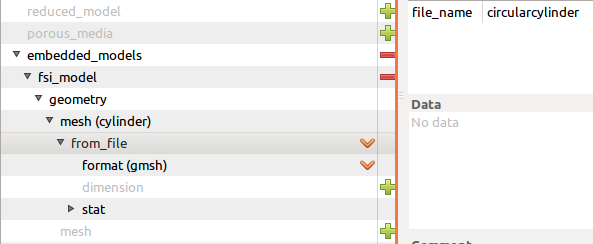
\includegraphics[scale=0.4]{content/diamond-setup/images/diamond-embedded-models-solid-mesh}}}
  \only<5-6>{\item FSI Projection}
  \only<5>{\\\fbox{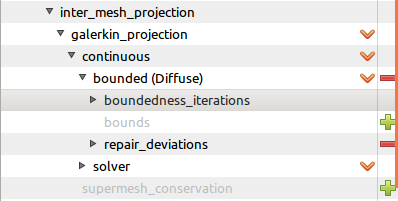
\includegraphics[scale=0.4]{content/diamond-setup/images/diamond-fsi-projection}}}
  \only<6>{\item Solid phases/fields}
  \only<6>{\\\fbox{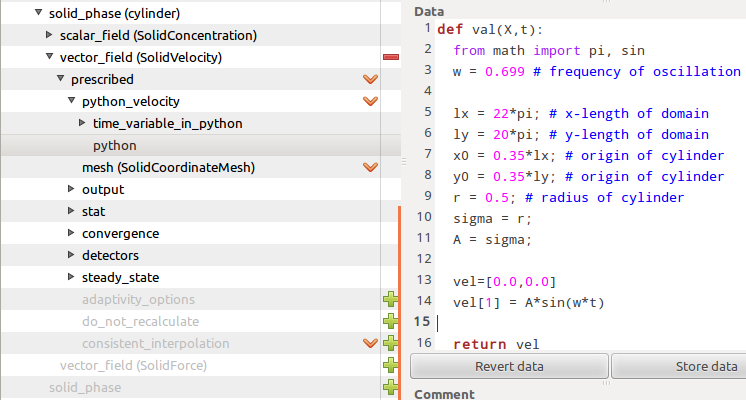
\includegraphics[scale=0.25]{content/diamond-setup/images/diamond-fsi-solid-phase}}}
 \end{itemize}
\end{frame}

\begin{frame}{Prescribed Velocity}
 To give a solid mesh a prescribed velocity, we have to use the Python function under the corresponding solid phase in diamond. Here: Oscillating cylinder\\
\begin{center}
\fbox{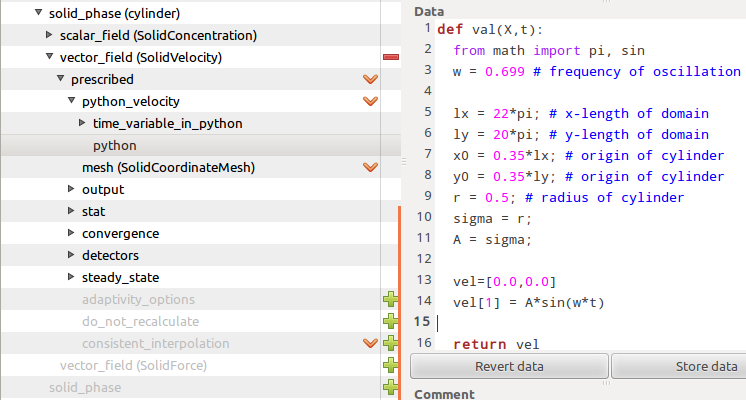
\includegraphics[scale=0.25]{content/diamond-setup/images/diamond-fsi-solid-phase}}
\end{center}
\end{frame}

\begin{frame}{Prescribed Velocity}
 Ellipse moving through a fluid, with positive and negative acceleration phases:
\begin{center}
\fbox{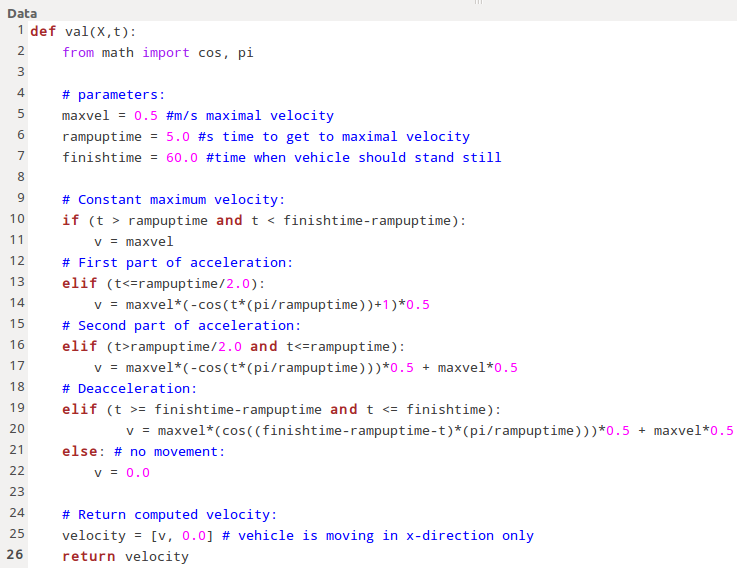
\includegraphics[scale=0.2]{content/diamond-setup/images/diamond-fsi-prescribed-velocity-ellipse}}
\end{center}
\end{frame}

\begin{frame}{Prescribed Velocity --- Rotations}
%  Prescribed Velocity/Movement, e.g.~rotational bodies
\vspace{-3ex}
\begin{center}
\only<1>{\fbox{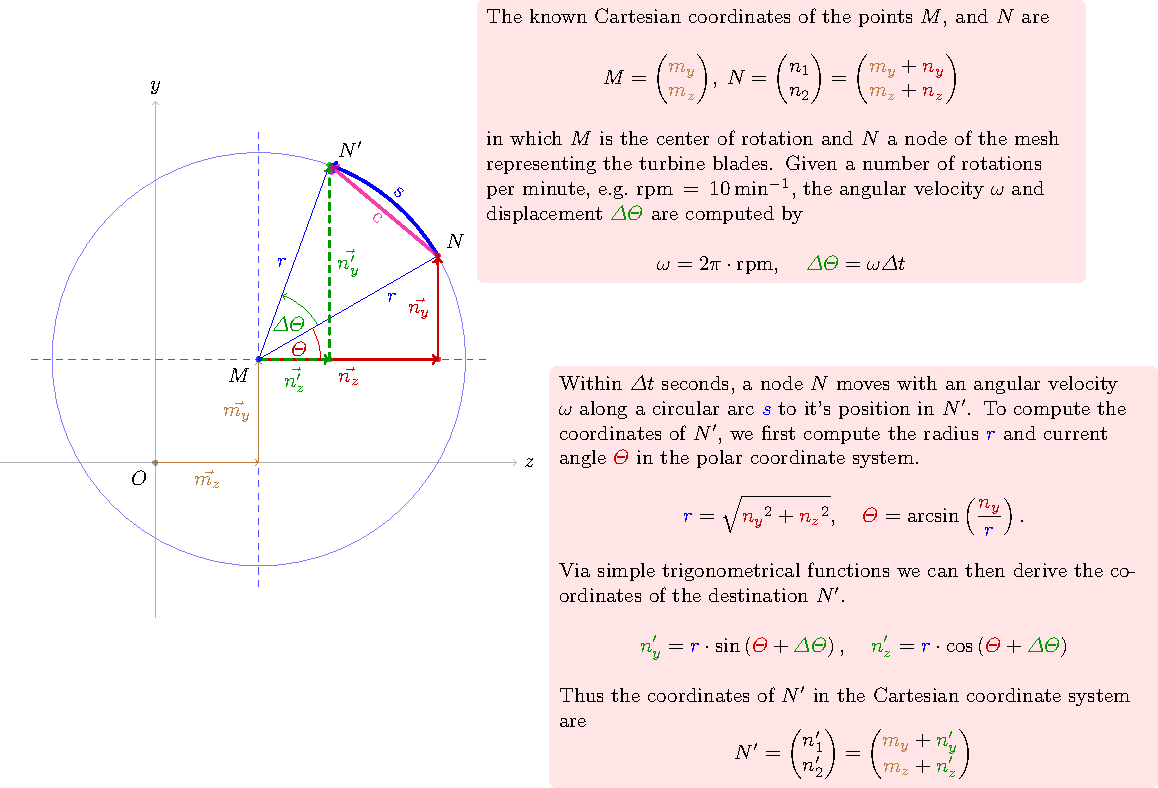
\includegraphics[scale=0.45]{content/schematic/1way_coupling_prescribed_rotation}}}
\only<2>{\fbox{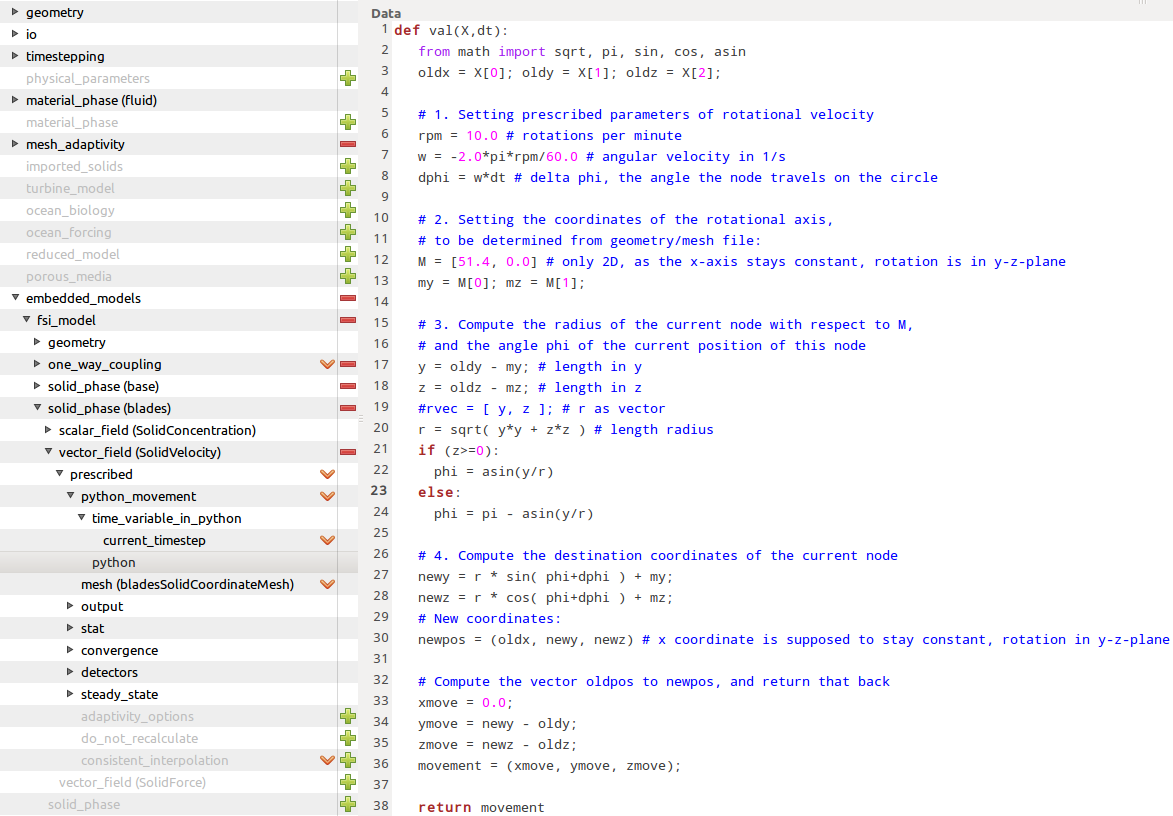
\includegraphics[scale=0.2]{content/diamond-setup/images/diamond-fsi-prescribed-velocity-turbine-blades}}}
\end{center}
\end{frame}



%%%%%%%%%%%%%%%%%%%%%%%%%%%%%%%%%%%%%%%%%
% Output                                %
%%%%%%%%%%%%%%%%%%%%%%%%%%%%%%%%%%%%%%%%%
\section{FSI Output}
\begin{frame}{FSI Output}
 \begin{itemize}
  \item Solid vtu files (serial)\\
    {\scriptsize\textbf{\color{blue}Fluid:} \textsl{simbasename}\_i.(p)vtu\footnote[4]{i corresponds to the vtu dump number}} \\
    {\scriptsize\textbf{\color{red}Solid:} \textsl{simbasename}\_solid\_\textsl{solidmeshname}\_i.vtu\footnote[5]{solidmeshname: name set in the flml for a solid mesh file}}
 \only<2-3>{
  \item Solid checkpoints (serial)\\
    {\scriptsize\textbf{\color{blue}Fluid:}  \textsl{simbasename}\_CoordinateMesh\_i\_checkpoint\_j.msh\footnote[6]{In a parallel run j is the corresponding MPI process number}}\\
    {\scriptsize\textbf{\color{red}Solid:}\\\textsl{simbasename}\_solid\_\textsl{solidmeshname}SolidCoordinateMesh\_i\_checkpoint.msh}
 }
 \only<3>{
  \item Solid stat file (will be added in future)
 }
 \end{itemize}
\end{frame}


\end{document}
